% Online Resource 1 (Electronic Supplementary Material) of the manuscript.
% Shared by both front ends: paper/emse/esm.tex typesets it as its own document
% (Springer's "Online Resource 1", sections A, B, C...), and paper/paper.tex
% inputs it after \appendix so the Elsevier fallback stays complete.
% Everything here was moved out of body.tex when the article was cut to length;
% the article keeps a summary of each part and points here.
% Unlettered references (Section 6.4, Table 4) are to the article; in the EMSE
% build they resolve through xr-hyper against paper/emse/main.aux.
%%%%%%%%%%%%%%%%%%%%%%%%%%%%%%%%%%%%%%%%%%%%%%%%%%%%%%%%%%%%%%%%%%%%%%%%%%%%%%%
\section{Related work: the comparison table}
\label{app:related}

Table~\ref{tab:related} places this study against the work closest to it on the
two axes that matter here: how many language ecosystems are compared, and how
energy is measured. Section~\ref{sec:related} discusses the studies that
deserve more than a row.

\begin{table*}[t]
\centering
\caption{The closest prior work, on the two axes this study varies. ``Stacks''
counts distinct language--framework combinations compared under one protocol.}
\label{tab:related}
\begin{tabularx}{\linewidth}{@{}l >{\raggedright\arraybackslash}X l >{\raggedright\arraybackslash}X l@{}}
\toprule
\textbf{Study} & \textbf{Stacks} & \textbf{Hardware} & \textbf{Energy instrument} & \textbf{Replication} \\
\midrule
\citet{li2016evaluating} & 4 frameworks, Python only & CPU + GPU & external meter & repeated \\
\citet{pereira2021ranking} & 27 languages, no DL & CPU & RAPL & 10 runs \\
\citet{gordillo2024ranking} & 8 languages, no DL & CPU & hardware meter & repeated \\
\citet{georgiou2022green} & 2 frameworks, Python only & CPU + GPU & RAPL + NVML & 30 runs \\
\citet{alizadeh2024energy} & 4 runtimes, Python only & CPU + GPU & software estimator & repeated \\
\citet{li2024bindings} & 5 bindings, 2 frameworks & CPU + GPU & none (time, memory, accuracy) & repeated \\
\citet{jay2023experimental} & software meters, not stacks & CPU + GPU & meters against a wattmeter & repeated \\
\citet{marini2025green} & 5 languages & CPU + GPU & software estimator & single run \\
\citet{chattaraj2025rvspython} & 2 languages, no DL & CPU & software estimator & repeated \\
\midrule
This study & \vEcosystems{} stacks, 5 languages & CPU + GPU & NVML + RAPL counters, estimator alongside & \vRepetitions{} runs \\
\bottomrule
\end{tabularx}
\end{table*}

%%%%%%%%%%%%%%%%%%%%%%%%%%%%%%%%%%%%%%%%%%%%%%%%%%%%%%%%%%%%%%%%%%%%%%%%%%%%%%%
\section{Research methodology, in full}
\label{app:methodology}

This section gives the parts of Section~\ref{sec:methodology} that the main text
condenses: the precision policy as implemented, the specification clause by
clause, the history of its conformance checks, the residual divergences, and the
detail of the measurement procedure.

\subsection{The precision policy as implemented}
\label{app:precision-policy}

All \vEcosystems{} ecosystems run under one precision policy, and it is set
rather than inherited: fp32 storage and arithmetic, with TF32 permitted on the
accelerator's tensor cores for convolution and for matrix multiplication. For
convolution that is what cuDNN does on this hardware unless it is told
otherwise, so it is the path a practitioner measures without choosing it; for
matrix multiplication it is not, since every binding leaves that path at fp32 by
default, and we state both halves rather than set one and inherit the other. A
single variable carries the policy --- \code{DEEPGREEN\_TF32}, applied through
the frameworks for the stacks that import our harness and through
\code{NVIDIA\_TF32\_OVERRIDE} for the four processes that never do --- and every
run's manifest records the flags that resulted. Setting it to \code{0} denies
TF32 to all \vEcosystems{}. Mixed precision is a separate axis and is enabled in
no stack here.

The policy belongs to the specification of Section~\ref{subsec:spec} rather than
to each ecosystem, and it is there because of what happened when it was not. A
first execution of this campaign pinned TF32 \emph{off} in the shared harness;
the pin reached one stack of \vEcosystems{} and no other, and that single
difference was worth more than any difference between bindings this study
measures. Section~\ref{app:tf32} reports it as an ablation.

\subsection{The specification, clause by clause}
\label{app:spec}

A fixed-budget comparison presumes that the budget is the same. In practice each
ecosystem is written by a different person against a different API, and the
places where they can silently diverge are numerous, individually reasonable and
invisible in the energy output: a default learning rate that differs between two
framework APIs, a data loader whose worker count follows the machine rather than
the protocol, an evaluation loop written one image at a time because the API
made that natural, an input tensor left at its native resolution in one stack
and resized in another.

We therefore wrote the protocol down before running anything, as a
specification with six parts, and made conformance machine-checkable. A seventh
part, added before the cell it governs was run, declares the one contrast
experiment outside the campaign.

\begin{itemize}\itemsep2pt
  \item \textbf{S1 --- Model.} One canonical definition per architecture.
        \texttt{scripts/export\_torchscript\_models.py} exports one TorchScript
        module per (architecture, dataset) pair, and
        \texttt{models/MANIFEST.json} records that module's parameter count and
        a hash of the parameters in name order. The \vCtrlStacks{} ecosystems that share the
        pinned LibTorch build (Python/PyTorch, C++, Rust) load that module; the
        remaining stacks build the same architecture in their own framework,
        from the same initialiser and the same batch-normalisation convention,
        because a framework's defaults for either are not a property of the
        ecosystem a reader is asking about. The manifest's parameter count is
        carried into every run as \texttt{DEEPGREEN\_EXPECTED\_PARAMS}, and the
        three Python stacks, R and Java assert it at startup and refuse to train
        if it does not match. C++ receives it and does not check it, and neither
        do the Rust binaries of the $32\times32$ campaign; the Rust binaries
        written for the saturation cell of S7 do. We found this after both
        campaigns had run, and we report it rather than patch a harness that has
        already produced the data. C++ and Rust load the same exported module
        file as PyTorch, which does assert it, so what they lack is the startup
        assertion, not a verified architecture. Counting parameters is the weak form of the check --- two
        networks can agree on a total and differ layer by layer --- so
        \texttt{scripts/verify\_architecture\_parity.py} builds each stack's
        model for every cell and compares the sorted multiset of parameter
        tensor shapes, which is comparable across languages where names and
        orderings are not: all \vEcosystems{} stacks agree, shape for shape, on
        all six cells. R links a LibTorch of its own and its binding cannot
        switch a script module between training and evaluation mode, so it
        builds the architecture rather than loading the module; it belongs to
        the LibTorch lineage but not to the control group. In an earlier version
        of this study this clause asserted the parameter check and nothing
        implemented it;
        Section~\ref{app:catalogue} records what that cost, and the C++ and
        Rust gap above is where it is still not implemented.
  \item \textbf{S2 --- Optimisation.} One optimiser, one learning rate, one
        batch size, one epoch count, one loss and one seeding policy. The
        learning rate and the batch size are checked against the source of every
        file the campaign executes --- universally, rather than by finding one
        file that matches; the rest is asserted by the specification and was
        checked by reading.
  \item \textbf{S3 --- Pipeline.} One input specification: $32\times32\times3$
        images in raw $[0,1]$ with no per-stack normalisation, resized once
        offline so that no framework's resampler enters the comparison; a
        bounded and equal number of loader workers; batched evaluation at the
        training batch size; and the whole 10,000-image test split evaluated in
        every stack, with no final partial batch dropped and no step count
        rounded down. Every run writes a fingerprint of the split it decoded ---
        mean, standard deviation and range over its \vDataFpValues{} pixel
        values --- so the pipelines are demonstrated to agree rather than
        asserted to.
  \item \textbf{S4 --- Backend.} One LibTorch build across the \vCtrlStacks{}
        stacks that share it, and one precision policy for all \vEcosystems{}:
        fp32 storage, TF32 allowed, stated to the CUDA libraries campaign-wide.
        The accelerator is asserted against the built artefact and not only
        against the source: \texttt{readelf -d} on every Rust binary we build
        must show a CUDA library among its \texttt{NEEDED} entries, and the
        harness refuses to start on a CPU device rather than warning about it.
  \item \textbf{S5 --- Measurement.} One measurement bridge, one sampling
        interval, one tracking mode, one set of counters, one unit, and one
        per-epoch record --- training loss, test loss and test accuracy ---
        persisted by every stack alongside energy, checked against the
        campaign's own metric files rather than against the source that writes
        them. Training accuracy is recorded by the \vTrainAccStacks{} stacks
        whose training loops already compute it, and is read by no analysis in
        this paper; the schema names those stacks rather than implying
        \vEcosystems{}.
  \item \textbf{S6 --- Replication.} Each configuration is executed
        \vRepetitions{} times as independent processes with distinct seeds,
        interleaved rather than run back to back. The seed is threaded from the
        run contract into each stack's data order and its initialisation, and
        two of the three ways a stack can ignore the seed it is handed are now
        checked against the stacks' source rather than against the campaign
        planner alone.
  \item \textbf{S7 --- Accelerator-saturation cell.} One declared contrast
        cell, run apart from the campaign and never pooled with it. S1, S4, S5
        and S6 hold as written --- the same \vSatEcosystems{} stacks, the same
        two architectures exported once as ten-class modules, the same
        instruments and \vSatReps{} interleaved repetitions. S2 keeps Adam at
        $1\times10^{-4}$ for \vSatEpochs{} epochs and changes the batch size,
        to 32 in training and evaluation alike. S3 changes the data: Imagenette,
        ten ImageNet classes, resized once offline to $224\times224$ (shorter
        side, then a centre crop). Section~\ref{app:saturation-exec} gives the reasons for each
        deviation.
\end{itemize}



The specification is enforced by \vConformanceChecks{} automated checks that
read the source of every ecosystem, the configuration of every tracker, the
built binaries and the campaign's own metric files, and fail the build when a
stack drifts out of conformance. This matters more than it may appear.
A specification that lives only in a paper is a description of intent; the same
specification expressed as an executable check is a property of the artefact,
and it fails at the moment of the divergence rather than at peer review.
\vDefectOurs{} of the defects catalogued in Section~\ref{app:catalogue} were
introduced by us while building or repairing this study; most were caught by a
mechanism rather than by inspection, and two were not, which is the subject of
what follows. Several are now enforced by checks under S1, S3 and S5, so the
same divergence cannot recur.

\subsection{What the checks caught, and what they could not}
\label{app:checks}

Of the
\vConformanceChecks{} checks, \vConformancePassing{} pass and
\vConformanceFailing{} fail. That is not the interesting number, and we would
not report it on its own. Building the current suite meant first discovering
that several of its checks could not fail. The learning-rate check was
existential where the specification is universal: it passed when one file in a
glob matched, so one stack's check passed while four sibling files carried other
learning rates, citing as its evidence a file the campaign does not execute --- a
reader who set \texttt{lrAdam = 1e-2} and \texttt{batchSize = 999} in the
classes that do run still got \texttt{[ok]}. A guard on the output directory
could fail only in the case where the check before it had already failed. And the
device check verified that a definition string appeared in a source file, which a
binary with no CUDA library linked into it satisfies perfectly. The first is
universal now and the second resolves both paths against a temporary directory,
and each fails on the defect that motivated it; the device clause keeps its source
check and has gained an artefact check beside it. We report this
rather than quietly regenerating a count, because a specification whose checks
are relaxed until they pass is a description of intent again --- and a check that
cannot fail is the same thing with a green light on it.

The limit is sharper than that, and the campaign is what found it. The suite
proved that the architectures matched, that the pixels matched and that the
protocol matched, and none of that requires the code to run. Fifteen hours into
the campaign \vLateRuns{} runs had failed and all of them were the same
ecosystem and architecture: \vLateEcosystems{} training VGG-16 raised \texttt{flax.errors.InvalidRngError} on its first batch,
because the shared classifier head carries a dropout layer and that stack's
training step never handed it a random stream. The parameter count it had
already asserted was correct, since dropout has no parameters, and every check
we had added for this campaign passed. A conformance suite built from source text cannot
establish that a stack takes one step; only running it can. We fixed the defect
and replayed those runs (Section~\ref{subsec:measurement}), and we keep the
lesson rather than the embarrassment: static enforcement is a floor, not a
ceiling, and the campaign is part of the apparatus that checks the campaign.

\subsection{Residual, documented divergences}
\label{app:divergences}

Three divergences could not be removed and are
reported rather than hidden. First, Deeplearning4j 1.0.0-M2.1 is the last
release of its API and links against the CUDA 11.6 runtime, so the Java stack
cannot be brought onto the CUDA 12 toolchain the other six share. Second, and
more consequentially, that stack resolves its convolutions without cuDNN and
cannot do otherwise at this version: they go through nd4j's own im2col and
cuBLAS. \texttt{readelf -d} on \texttt{libnd4jcuda.so} shows a \texttt{NEEDED}
entry for cuBLAS and none for cuDNN, and the cuDNN convolution helper has no
release at any version, so nothing in the stack can call the cuDNN libraries its
own redistributable ships. The specification document in the replication
package carries the rest of the evidence. It is the only stack of \vEcosystems{} that
reaches no cuDNN kernel, and a conformance check now watches that library and
fails if a future version gains one, so the claim cannot quietly stop being true.
Because it cannot be fixed, we bound it: disabling cuDNN in a stack that has it,
holding hardware, model and data constant, costs
\vCudnnOffEnergyRatio$\times$ the energy and \vCudnnOffTimeRatio$\times$ the
time on ResNet-18 at batch 128. That is an upper bound on what losing cuDNN can cost
rather than an estimate of this stack's own penalty --- nd4j's im2col path is not
PyTorch's non-cuDNN fallback --- but it is large enough that Java's cost in this
study is in part a statement about a missing convolution backend rather than
about a language, and we repeat the qualification wherever that cost is reported.
Third, the R \texttt{torch} binding cannot switch a script module between
training and evaluation mode, so R alone cannot consume the shared TorchScript
module of S1 and builds the same architecture instead; its shapes are verified
against the other six inside the campaign environment, which is the only place
its binding loads. All three are properties of the ecosystems, and arguably part
of what one measures when one measures an ecosystem; we name them because a
reader deciding what a cost should be attributed to needs to know which of them
are in play.

\subsection{Measurement procedure, in detail}
\label{app:measurement}

The two halves of that sum are not at the same boundary, and the sum is not
``the chip''. NVML's register is a \emph{board} quantity: it includes the GPU
die, its GDDR6X and the card's voltage regulators. RAPL's package domain is the
CPU package alone. Host DRAM is in neither --- this platform exposes no
\texttt{dram} RAPL domain, so its energy, of order ten watts, is not measurable
here and is absent from every figure we report. We name the quantity
board-and-package rather than chip-level, and we note the asymmetry with our
own criticism of the estimator's modelled RAM term: that term is unverifiable,
and ours is missing altogether.

\texttt{CodeCarbon}~\citep{codecarbon} runs over the same window as
a second reading, in machine tracking mode at a one-second
sampling interval and the default \code{api\_call\_interval} of
\vMechApiCallInterval{}, configured identically for all \vEcosystems{} stacks
through a single shared bridge. We name that last parameter because
Section~\ref{subsec:rq3} shows it is the one that decides whether a reported
duration is a duration. The four non-Python ecosystems drive that bridge over a
line protocol with synchronous acknowledgement, so that a phase boundary in the
measured process and the corresponding counter read cannot drift apart;
Section~\ref{app:bridge} says what an asynchronous version of it cost.



\textbf{Replication and the unit of analysis.} Each of the \vConfigurations{}
configurations is executed \vRepetitions{} times as an independent process with
a distinct seed, giving \vRuns{} runs. \vInterleavedRuns{} of them ran
\emph{interleaved} rather than consecutively, so that drift in machine state ---
thermal, background, driver clock behaviour --- is spread across conditions
instead of aliasing onto whichever ecosystem happened to run last. The remaining
\vLateRuns{}, all \vLateEcosystems{} on VGG-16, are the runs the dropout defect
above stopped at their first batch; they were replayed \vLateGapDays{} days later
on the same host, and they are the one place where interleaving does not hold.
Section~\ref{sec:threats} reports what a between-window calibration says that is
worth. All uncertainty we
report is between-run: the 30 epochs within a run share an initialisation, a JIT
outcome, an allocator state and a thermal trajectory, and treating them as
repeated measurements would understate uncertainty while inflating apparent
significance.



\textbf{Reproducibility and rigor.}
Each run receives a seed from the run contract, and that seed reaches both the
data order and the model initialisation in every stack. Two of the three ways a
stack can ignore the seed it is handed are now checked against the stacks' own
source, which is two more than an earlier version of this study checked: in an
earlier campaign of this design
\vSeedDivergentStacks{} stacks of \vEcosystems{} were handed a distinct seed per
repetition and did not use it --- one hardcoded its shuffle seed, so all
\vRepetitions{} repetitions saw the same data order; one never forwarded the seed
to its loader; and one rebuilt its generator inside the epoch loop and replayed a
single permutation for every epoch --- while the conformance check reported five
distinct seeds, having asked the campaign planner rather than the stacks.
Initialisation is no longer each framework's default either: under S1 every stack
draws convolutions and dense layers from the same distributions, because a
default initialiser is not a property of the ecosystem this study is asking
about.
Nevertheless, full determinism cannot be guaranteed across all stacks due to non-deterministic GPU kernels and differences in backend execution engines; this is one reason the design replicates rather than relying on a single execution per configuration.

A complete replication package is provided (see replication package link in Section~\ref{sec:intro}), including: (i) source code for all implementations, (ii) scripts to reproduce runs, (iii) environment specifications (e.g. virtual environments, Maven, CMake), and (iv) collected raw data~\citep{cruz2025greening,verdecchia2023systematic}.
Configurations are standardized across languages where feasible, with deviations documented when framework-specific requirements arise~\citep{pereira2021ranking,gordillo2024ranking}.
This package enables replication, validation, and extension under different hardware or software conditions~\citep{feldt2010validity,sjoberg2023construct}.

%%%%%%%%%%%%%%%%%%%%%%%%%%%%%%%%%%%%%%%%%%%%%%%%%%%%%%%%%%%%%%%%%%%%%%%%%%%%%%%
\section{Experimental execution, in full}
\label{app:execution}

This section gives the execution detail that Section~\ref{sec:execution}
condenses.

\subsection{Platform}
\label{app:platform}

Section~\ref{sec:execution} describes the workstation.

Two properties of this platform bear directly on the measurements. First, both
energy counters are available: the RTX 3090 exposes NVML's accumulated-energy
register, and the Ryzen's package-energy counters are readable through the Linux
\texttt{powercap} interface --- which, for historical reasons, presents AMD
domains under \texttt{intel-rapl} names. We read the package domain and handle
counter wraparound at \texttt{max\_energy\_range\_uj} explicitly. Second, this is
a desktop rather than a server: it has one accelerator, one CPU socket and an
order of magnitude less RAM than a datacentre node, which is precisely why the
modelled RAM term discussed in Section~\ref{sec:instrument} is a smaller share
of a software estimator's total here than it would be on a large-memory host.

We report this as a replication platform rather than as the platform. The
campaign behind an earlier version of this study --- the \emph{audited
campaign}, as we call it throughout --- ran on a dual-socket Intel Xeon Gold 5418Y server
with an NVIDIA L40S; absolute energy figures are not comparable between the two
machines, and none of the comparisons in this paper is made across them. What
carries over is the design, the specification and the instrument
characterisation, all of which are properties of the method rather than of the
host.

\subsection{Model implementations and toolchains}
\label{app:implementations}

Every ecosystem trains the same architecture, and the stacks whose backend
permits it train the same artefact. Under specification S1 the \vCtrlStacks{}
stacks on the pinned LibTorch build --- Python/PyTorch, C++ and Rust --- do not
build \vCtrlStacks{} independent ResNet-18s and VGG-16s but load one TorchScript
module per (architecture, dataset) pair, exported once by a single script and
recorded in a manifest with its parameter count and a hash of the parameters in
name order. The
other four build the same definition in their own framework and assert that count
at startup against the same manifest, as does PyTorch; C++, and Rust in the
$32\times32$ campaign, do not (Section~\ref{subsec:spec}), and a parity script compares all
\vEcosystems{} stacks on the sorted multiset of their parameter tensor shapes
rather than on a total. That last distinction is not pedantry. In an earlier
campaign of this design the stacks were compared on parameter counts that nothing
checked, and VGG-16 ran as four different networks spanning an order of magnitude
in parameters under one name; comparing them was comparing models, not
ecosystems.

Table~\ref{tab:frameworks} lists the versions. The Python stacks are installed
in three separate virtual environments rather than one, because their CUDA and
cuDNN wheels conflict: a shared environment resolved to a cuDNN that TensorFlow
could not dlopen, and TensorFlow then ran unaccelerated while reporting only a
warning --- a failure mode the accelerator assertion of S4 now turns into an
error at startup. The assertion by itself was not enough. A binary can satisfy
any source-level device check and still have no CUDA library linked into it,
which is what happened to our own Rust stack for a day, so S4 is checked against
the built artefact as well: \texttt{readelf -d} on every released Rust binary,
which immediately found two stale ones.

\emph{Toolchain divergence, and what is left of it.} The \vCtrlStacks{}
stacks of the control group are pinned to one LibTorch build (2.7.0, CUDA 12.8),
so within it the backend is genuinely held constant. Four of the
\vEcosystems{} ecosystems cannot join them, for three different reasons. TensorFlow and JAX
bring their own backends and are not LibTorch stacks at all.
Deeplearning4j 1.0.0-M2.1 links against the CUDA 11.6 runtime, resolves its
convolutions without cuDNN, and has had no subsequent release; the stack now
carries its own redistributables through
\texttt{org.bytedeco:cuda-platform-redist}, which makes it reproducible without
making it contemporary, and Section~\ref{subsec:spec} bounds what the missing
convolution backend can be worth. R's \texttt{torch} 0.17.0 bundles its own
LibTorch and
resolves CUDA at load time. We report these as documented divergences rather
than normalising them away, and Section~\ref{subsec:rq1} reports the LibTorch
control group separately so that a reader can see how much of the total spread
survives when the backend is held fixed.



During a preliminary pilot phase, the Julia programming language (using \texttt{Flux} and \texttt{Lux}) was also considered. However, persistent technical challenges encountered during implementation related to gradient updates during training, which remained unresolved also after directly contacting the developers of the libraries, prevented its reliable inclusion in the final study.

\subsection{The saturation cell as executed}
\label{app:saturation-exec}

Specification S7 adds one contrast cell, executed
after the campaign and on the same host:
Imagenette\footnote{\url{https://github.com/fastai/imagenette}}, ten easily
separated ImageNet classes, 9,469 training and 3,925 test images, resized once offline by the
shorter side to 224 and centre-cropped to $224\times224$ so that, as in the
campaign, no stack's resampler enters the comparison. Three rows of
Table~\ref{tab:hyperparams} differ for the cell: input resolution; batch size,
32 in both phases, because VGG-16 at $224\times224$ does not fit the card's
24\,GB at batch 128 --- a hardware limit, not a preference; and evaluation, which
still batches at the training batch size but covers the 3,925-image test split.
The classifier has ten outputs, as on Fashion-MNIST, so the parameter counts the
stacks receive are that pair's. The
cell is \vSatEcosystems{} ecosystems $\times$ \vSatModels{} architectures
$\times$ \vSatReps{} repetitions, \vSatRuns{} runs of \vSatEpochs{} epochs,
interleaved repetition-major under the same fixed shuffle. S7 allows the
loader-worker count to be raised at this resolution and requires it to be
recorded per run; it was not raised, and every run of the cell records the same
\vSatLoaderThreads{} workers as the campaign. The cell lives in a campaign directory of its own:
the driver refuses to schedule it into the campaign's directory or alongside the
$32\times32$ datasets, the campaign's directory and every table derived from it
are frozen, and the analysis writes the cell's tables to a separate location. The
two differ in resolution, batch size and class count, so no figure in this paper
aggregates across them; Section~\ref{sec:saturation} reports the cell as a
contrast, and every comparison there is computed the same way on both sides.

\subsection{Measurement and the shared bridge}
\label{app:bridge}

Each phase of each epoch is bracketed by two counter reads --- NVML's
accumulated-energy register and the CPU package RAPL counter --- and is
simultaneously tracked by \texttt{CodeCarbon} v3.3.0~\citep{codecarbon}. The two
are started and stopped by the same code path, so the intervals they
\emph{accumulate over} cannot drift apart. The counter reads are nested
immediately inside the tracker's, which costs a fixed offset we quantify in
Section~\ref{sec:instrument} rather than assume away. The interval CodeCarbon
\emph{reports} is a different thing again, and Section~\ref{subsec:rq3} is
about that.

The four non-Python ecosystems drive the instrumentation through a single shared
bridge: a Python process that accepts \texttt{START}, \texttt{STOP},
\texttt{METRIC} and \texttt{EXIT} over a line protocol, reads the counters, and
acknowledges each command before the measured process proceeds. The
acknowledgement is not incidental. An earlier, asynchronous version of the same
bridge allowed a phase boundary in the measured process to run ahead of the
corresponding counter read, which under-reported one stack's training energy by
24\% and recorded its evaluation energy as exactly zero --- a value that looks
like a bug only if someone thinks to look at it.

Running the bridge out of process also isolates the measured stack from the
instrument: a crash in the tracker cannot take down a six-hour training run. It
does not remove the tracker's own cost from the measurement --- under
whole-machine tracking its once-per-second sampling runs inside the block and
its package energy is inside the block's RAPL delta. That cost is a constant per
second and identical for every stack, so it does not bias the comparison, but it
is inside the numbers and we would rather say so. All runs execute in isolation on an otherwise idle
host, as whole-machine tracking requires, and each block is logged with dataset,
model, ecosystem, repetition, seed, phase, epoch, both energy readings, the
duration and the test accuracy reached.

\subsection{Reproducibility artefacts and their limits}
\label{app:repro}

A comprehensive replication package accompanies this study (see the link in
Section~\ref{sec:intro}). Beyond source code, automation scripts, per-ecosystem
environment specifications and raw logs, it contains three artefacts specific to
this design:
\begin{enumerate}[label=(\roman*)]
    \item the \textbf{experiment specification} of Section~\ref{subsec:spec},
          written before the campaign and versioned with it;
    \item the \textbf{conformance checker}, \vConformanceChecks{} executable checks that read the
          source of every ecosystem and the configuration of every tracker, and
          fail when a stack drifts out of specification;
    \item the \textbf{dual-instrument records}: every block's counter reading
          and estimator reading side by side, which is what makes the analysis
          of Section~\ref{sec:instrument} reproducible rather than anecdotal.
\end{enumerate}
Every quantity this manuscript reports from the campaign is generated from
those records by the analysis pipeline and injected into the source at build
time. The exceptions are stated where they occur: figures recovered from the
audited campaign, and one-off diagnostics reproduced from the record
that established them. Two limits on that provenance are worth stating rather
than leaving for a replicator to find. Every run's manifest records the machine
state it ran under --- driver, power limit, clocks, persistence mode, governor,
boost and the precision policy in force --- but every run of this campaign
predates the harness-provenance field and so carries machine state without a
source revision; the field is recorded from the next campaign on. And the
analysis used to write its tables into the directory the manuscript reads, so a
monitoring pass over a campaign still in flight briefly replaced the campaign's
own run count with a partial one; the pipeline now diverts to a separate
directory until the expected number of runs is complete. Neither changes a number
reported here, and both are the kind of thing a reproducibility claim has to be
able to survive being asked about.

\subsection{The configuration, and what verifies it}
\label{app:config}


The configuration is in Table~\ref{tab:hyperparams} of the article. Of its rows, the learning rate and the batch
size are verified against the source of every file the campaign executes,
universally rather than by one file that happens to match; the precision policy
is verified as a campaign-wide export and by a negative check that no stack pins
it privately; the other rows are asserted by the specification and were checked
by reading. Section~\ref{app:checks} reports why that distinction is not
pedantic. Each block is logged with dataset, model, ecosystem, repetition, seed,
phase, epoch, both energy readings, the duration and the test accuracy reached
(Section~\ref{app:bridge}). Section~\ref{subsec:rq1} reports the LibTorch
control group separately so that a reader can see how much of the total spread
survives when the backend is held fixed.

%%%%%%%%%%%%%%%%%%%%%%%%%%%%%%%%%%%%%%%%%%%%%%%%%%%%%%%%%%%%%%%%%%%%%%%%%%%%%%%
\section{RQ1: supplementary analyses}
\label{app:rq1}

Section~\ref{subsec:rq1} answers RQ1 and summarises the analyses given in full
here: the training energy behind Figure~\ref{fig:energy_ci}, what an earlier
version of this study read into the control group,
the runs that collapsed in the first execution of this design, and the precision
policy that separated the two executions.

\subsection{Training energy per epoch, tabulated}
\label{app:train-energy}

Table~\ref{tab:train_energy} gives the means that Figure~\ref{fig:energy_ci}
plots, per ecosystem and cell; Table~\ref{tab:spread} in the article picks out
the cheapest and the dearest stack of each cell.

\begin{table*}[t]
\centering
\caption{Mean training energy per epoch (J), accelerator plus CPU package.}
\label{tab:train_energy}
\input{\gendir tab_train_energy.tex}
\end{table*}

\subsection{What an earlier version read into the control group}
\label{app:control}

An earlier version of this study read a mechanism out of Table~\ref{tab:libtorch_control}, and it was
wrong. It argued that whatever separates those three cannot be the kernels,
because the kernels are the same code, and it put about half of the ResNet-18
log spread under binding overhead, data movement and host-side dispatch. Sharing
a build is not sharing a kernel configuration. Specification S4 asked for fp32
with TF32 disabled, and exactly one stack of \vEcosystems{} was given it, the
other six taking cuDNN's Ampere default --- so the two campaigns hold that
ablation between them. Python/PyTorch's own ResNet-18 training energy is
\vPrecisionPytorchRatioMin$\times$ higher in the campaign that denied it TF32
than in this one, on \vPrecisionGapDataset{} --- the one cell the two campaigns
leave comparable --- while the \vPrecisionControlStacks{} stacks of that cell
whose precision policy did not change move by at most
\vPrecisionOthersMaxChangePct\,\%; an isolated kernel probe puts the same flag
pair at \vPrecisionKernelDetEnergyRatio$\times$ on the accelerator alone
(Section~\ref{app:tf32}). The
PyTorch-versus-C++ gap the earlier campaign measured there,
\vPrecisionGapBefore$\times$, is \vPrecisionGapAfter$\times$ in this one, and
it was nearly absent on VGG-16, whose classifier is GEMM rather than convolution
--- which no account of binding overhead predicts. Two further premises were
false: the three stacks did not begin from identical parameters
(Section~\ref{app:collapse}), and the stacks outside the group were not
all running the same network under the name VGG-16. All of that is fixed in the
campaign reported here. What we report from Table~\ref{tab:libtorch_control} is
the spread that survives holding the model and the backend build fixed. We do
not decompose what is left, because a black-box design of this shape cannot, and
the cost of guessing is on the record above.

\subsection{Runs that consumed the budget and learned nothing, and why none did here}
\label{app:collapse}

Replicating each configuration surfaced something a single run cannot show. In
the first campaign of this design VGG-16 did not always train. We call a run
\emph{collapsed} when its final test accuracy never exceeds
\vCollapseFactor$\times$ chance for its dataset; the multiplier is generous on
purpose, because every collapsed run sat at chance exactly --- 1/100 on
CIFAR-100, 1/200 on Tiny ImageNet --- so no case depends on where the line is
drawn. By that criterion \vCollapseFirstVgg{} of \vCollapseFirstVggRuns{} VGG-16
runs collapsed and stayed collapsed for all 30 epochs, having consumed the full
energy budget while learning nothing. ResNet-18 never does this in either
campaign --- \vCollapsedResnet{} of \vCollapsedResnetRuns{} runs in the campaign
reported here --- and neither architecture does it on Fashion-MNIST.

\begin{figure*}[t]
    \centering
    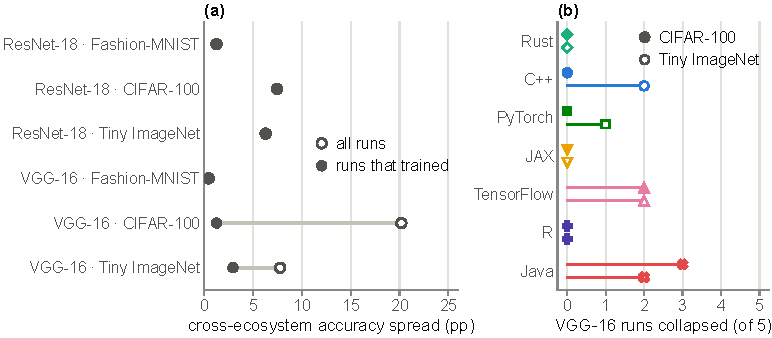
\includegraphics[width=\linewidth]{figures/fig_convergence_first_campaign.pdf}
    \caption{The superseded first campaign, from that campaign's own records.
    (a) Cross-ecosystem accuracy spread per cell, over all runs (hollow) and
    over only the runs that trained (filled); the gap on VGG-16 is the collapsed
    runs. (b) VGG-16 runs that collapsed to chance, out of \vRepetitions{} per
    cell, on CIFAR-100 (filled) and Tiny ImageNet (hollow). The same
    figure for the campaign reported here is not drawn: with
    \vCollapseRuns{} collapses its panel (a) plots one set of runs against
    itself and its panel (b) is empty in every cell.}
    \label{fig:convergence_first}
\end{figure*}

The per-epoch traces say precisely what those runs were. In every one of them
the loss sat at $\ln N$ for the $N$ classes of the dataset --- 4.605 on
CIFAR-100, 5.298 on Tiny ImageNet --- to within
\vCollapseFirstLossDeviationMax{}, for all thirty epochs. That is the loss of a
\emph{uniform} output distribution: the network is not confidently predicting
one class, it is producing the same distribution for every input, and no
gradient signal is reaching it. VGG-16 as shipped carries no batch
normalisation, and a plain sixteen-layer network driven by Adam at $10^{-4}$
over a hundred or two hundred classes can start there and never leave.

What decides whether a run does so is the initial weights. The previous
version of this section said the opposite, and the premise it rested on was
false: we argued that the \vCollapseSharedStacks{} stacks described as loading
a byte-identical exported module began from identical parameters and still
disagreed about which repetitions collapsed, so the deciding factor had to be
the stochastic path. They did not begin from identical parameters. Python's
PyTorch harness built torchvision's network fresh and loaded no module at all,
and the C++ and Rust harnesses each loaded a module from a separate, unseeded
export.

A controlled side experiment outside the campaign reverses the reading. VGG-16
on the many-class datasets, one framework, \vInitCollapseTrials{} runs per
initialiser, with framework, optimiser, learning rate and data order held
fixed and only the initialiser varied: \vInitCollapseHe{} runs collapse under
He initialisation, \vInitCollapseGlorot{} under Glorot and
\vInitCollapseXavier{} under Xavier. The stacks were not drawing from one
distribution and diverging afterwards; they were drawing from different
distributions. Deeplearning4j, the one stack with a hand-rolled initialiser
--- a truncated normal scaled by fan-in where torchvision scales, untruncated,
by fan-out, \vInitStemWidthRatioJava$\times$ wider at ResNet-18's $7\times7$
stem --- carried \vCollapseFirstJava{} of the \vCollapseFirstVgg{} collapses.
Those runs belong to neither campaign and no analysis script regenerates them;
they are preserved as a record in the replication package. What we reported as
a property of the ecosystems is a defect class about framework defaults:
VGG-16 without batch normalisation under Adam at $10^{-4}$ is
initialisation-critical, and frameworks ship different initialisers under the
same architecture name. An architecture name does not fix the network that gets
trained, and nothing in an energy table records which distribution a stack
drew from.

The campaign reported here removes the cause rather than the symptom. Every
stack starts from one canonical seeded export of each architecture, and the
stacks that build their own layers use initialisers matched to torch's. Under
that change VGG-16 collapsed \vCollapseRuns{} times in \vCollapsedVggRuns{}
runs. Zero events do not prove a zero rate: over the
\vCollapseSusceptibleRuns{} runs in the cells where collapse ever occurred ---
VGG-16 on the two many-class datasets --- the exact one-sided 95\,\% upper
bound on the rate is \vCollapseRateUpperNinetyFive\,\%, against the
\vCollapseFirstRateOverall\,\% measured on the same cells before. And with no
collapse in any ecosystem there is no table of rates to test: the exact test
of homogeneity returns $p = \vCollapseExactP$ because every cell is zero,
which makes it a statement about the table's shape rather than a test
(Section~\ref{app:threats} says why that test replaced the two we first ran).

\textbf{A failed recipe and a broken pipeline look identical in an energy
table.} Both produce chance accuracy at full energy cost, and neither is visible
in a Joule figure. The per-epoch traces separate them. In a genuine collapse the
training loss does not move either, because a network that has settled on a
uniform output has nothing left to fit. A pipeline defect looks the opposite:
the training loss falls normally while test loss \emph{rises} and accuracy stays
at chance, which says that training and evaluation are not seeing the same
inputs.

The diagnostic as we first built it could not do that for every stack, and we
did not notice. It conjoins the two arms, and our Java harness recorded
\code{NaN} for test loss in every one of its epoch rows; a comparison with
\code{NaN} is false, so the conjunction could never fire for Deeplearning4j ---
the stack carrying \vCollapseFirstJava{} of the \vCollapseFirstVgg{} collapses.
We described that as a diagnostic degrading to its remaining arm. It did not
degrade: Java's sensitivity to pipeline defects was zero rather than reduced,
and no Java run was ever tested by it. Test loss is now computed in the same
inference pass as accuracy, so both arms are live in all \vEcosystems{} stacks
and Java's evaluation blocks no longer measure twice the work.

We report this because the discriminator found a defect of our own that the
collapse count alone would have absorbed. \vDefectRuns{} runs met the
chance-accuracy criterion --- at most \vDefectAccMax\,\% --- with training loss
falling by \vDefectLossDropMin--\vDefectLossDropMax\,\%: one Rust binary carried
a private copy of the input transform, applied on the training path only, which
resized the tensor its loader had already produced using a function that returns
\code{uint8}. Every value in $[0,1]$ truncated to zero, so it trained on black
images and was evaluated on real ones. Filed as collapses they would have read
as ``VGG-16 sometimes fails to train''. Those runs were deleted and the
configuration re-executed; since the evidence for a defect should be as
traceable as the evidence for a result, and the discarded runs no longer exist
in the campaign, their signature is preserved as a record in the replication
package rather than quoted from memory.

The same defect class came back later in a different file, and what caught it
was not this diagnostic. When the datasets were pre-resized offline so that each
stack's own resize became a no-op, the \code{uint8} guard was written into one
of the three Rust loaders and not the other two, so the Fashion-MNIST loader
went on resampling an already 32$\times$32 image and its pixel statistics stayed
away from the other stacks' --- not far enough to reach chance accuracy, and so
invisible to a test that triggers on chance accuracy. It was found by comparing
pixel statistics across all \vEcosystems{} stacks. All three loaders are guarded
now. In the campaign as it stands the
discriminator finds \vSigPipelineN{} pipeline defects and \vSigCollapseN{}
collapses, which is what a campaign with nothing to separate looks like rather
than a claim that the class is closed.


We are able to state the discriminator's recall on the one instance we have,
and it is not perfect. The defect was a deterministic code path on the training
branch, so all \vRepetitions{} repetitions of that configuration carried it; the
discriminator flagged \vDefectRuns{}. The remaining run finished above the
collapse threshold and so was never a candidate for the test at all, and the
second instance of the same defect class --- the loader described above --- never
came near the threshold either. That is precisely why a discriminator triggering
on chance accuracy is a diagnostic aid and not a detector. One calibrated on a
single positive example, with a threshold chosen after seeing it, is a heuristic:
it separates the two failure modes cleanly once a run is known to have failed,
and it will miss a defect that leaves enough accuracy behind. We report it as the
diagnostic aid it is.

Two consequences matter here.

\textbf{The stacks agree on what they compute.} No cell shows a
cross-ecosystem accuracy spread above \vCondSpreadMax{} percentage points, and
the widest of them, on \vCondBlockName{}, is a spread between runs that all
trained. In the first campaign the same measurement had two arms --- over all
runs, and over the runs that trained --- and almost the entire apparent
disagreement between stacks sat in the gap between them
(Figure~\ref{fig:convergence_first}a). There is no gap now: every run in this
campaign trained, the two arms coincide, and the spread is what the stacks
compute rather than what failed to train.

\textbf{A collapse breaks fixed-budget energy comparison, invisibly.} A
collapsed run costs full energy and produces nothing: in the first campaign
\vCollapseFirstWastedPct\,\% of the training energy went on runs that learned
nothing, against \vWastedPct\,\% of the \vTrainingEnergyMJ~MJ spent here. An
ecosystem whose default initialiser differed from the recipe's looks equally
expensive and much less accurate; one whose default matched it looks efficient.
With a single run per configuration --- the design this study replaces --- the
reported number is whichever outcome that one configuration produced, and
nothing in the energy data distinguishes the two cases. This is why we report
accuracy alongside energy rather than assuming a fixed budget delivers fixed
quality.

\subsection{The precision policy, and what it was worth}
\label{app:tf32}

This campaign was executed twice, and the difference between the two executions
is a measurement. The first pinned TF32 off --- \code{cudnn.allow\_tf32} and
\code{matmul.allow\_tf32} false, \code{cudnn.deterministic} true --- in the
harness the Python stacks import. Only those three stacks import it, and of
those only PyTorch reached cuDNN through it: TensorFlow was handed a
mixed-precision policy, which is a different axis, and JAX was handed nothing.
So one stack of \vEcosystems{} trained true-fp32 convolutions while the other
six took cuDNN's Ampere default, which is TF32. The re-execution reported
throughout this paper runs all \vEcosystems{} under the single policy of
Section~\ref{subsec:spec}. Because the two executions differ in the precision
policy of exactly one stack, over the same \vConfigurations{} configurations,
they are between them an ablation of that policy against a control group whose
precision policy did not change, and we report them as one. (The audited campaign that
motivated this design, in Section~\ref{sec:catalogue}, is a different thing again
and ran on different hardware; nothing here is compared against it.)

Table~\ref{tab:precision_contrast} puts the two executions side by side, per
epoch of training, and says of every ResNet-18 training cell whether anything
other than the precision policy changed between them. On
\vPrecisionGapDataset{}, where nothing else did, Python/PyTorch's ResNet-18
training energy is \vPrecisionPytorchRatioMin$\times$ higher with TF32 denied
than with it allowed, while the \vPrecisionControlStacks{} stacks that are
comparable beside it --- C++, Rust and R, whose precision policy did not change
and whose remaining differences between the executions cannot move per-epoch
energy --- move by at most \vPrecisionOthersMaxChangePct\,\%. And the
quantity an earlier version of this study leaned on hardest, the
Python/PyTorch-versus-C++ training gap on ResNet-18, falls from
\vPrecisionGapBefore$\times$ to \vPrecisionGapAfter$\times$. Each side of that
comparison is \vRepetitions{} runs of thirty epochs, on real data, on the
instrument this paper uses throughout.

\input{\gendir tab_precision_contrast.tex}

Most cells are not a precision contrast, and the table says which and why. Three
of the six stacks that kept their policy are excluded for reasons of their own:
Python/TensorFlow ran a Model Garden ResNet-18 with a projection shortcut the
other stacks do not have and dropped its last partial batch, Java/DL4J built its
graph by hand with truncated convolution padding and a bias on every
convolution, and Python/JAX was measured through a window that did not force
completion in the first execution and does in this one. VGG-16 is excluded
entirely, since the first execution ran four different networks under that name,
so a VGG-16 ratio between the two executions is mostly architecture.
Fashion-MNIST and Tiny ImageNet were re-encoded to the common $32\times32$
resolution on disk between the two, so on those datasets every stack's loader
does different work; CIFAR-100 was already at that resolution and did not move.
One caveat survives inside the cells that remain, and we state it rather than
remove it: the first execution built PyTorch's ResNet-18 fresh from torchvision
and this one loads the exported module of S1, so PyTorch's ratio contains
whatever TorchScript execution is separately worth. The control group cannot
separate the two, because the other stacks loaded a module in both executions.
The ratio therefore bounds the precision effect from above, and we do not
partition it. The kernel probe below reports a larger ratio for the same flag
pair, and the two are not in tension: the probe measures accelerator energy per
step on a resident batch, where this figure is board-and-package per epoch and
carries the loader and the CPU package with it.

Underneath that contrast we ran a kernel-level probe on an idle host
(\code{scripts/probe\_tf32.py}): ResNet-18 built from the definition the campaign
exports, batch 128, one resident batch of synthetic input, and the flags set
directly. Synthetic input is the point rather than a compromise, since which
convolution algorithm cuDNN selects does not depend on what the pixels are, and
holding one batch resident takes the loader out of the comparison identically in
every cell. Every ratio here is against the configuration the other six stacks
ran in the first execution: TF32 allowed to cuDNN, determinism unpinned, the
matrix-multiply path at its framework default of fp32 --- the cuDNN-disabled
cell excepted, which is taken against this campaign's own default, the only
configuration whose matrix-multiply flag it shares. A thousand training steps
per measured window (three hundred for the cuDNN-disabled cell) clears the \SI{5}{\second} floor the script enforces against
an NVML energy register that advances about ten times a second on this device
(Section~\ref{sec:instrument}), so these ratios are not quantisation-bound; the
cells are reshuffled from a recorded seed within each repeat, so drift over the
run cannot alias onto one of them, and we report medians over the repeats.
Denying TF32 to the convolutions costs \vPrecisionKernelEnergyRatio$\times$ the
accelerator energy per step. Denying it and pinning \code{cudnn.deterministic}
as well --- the first execution's configuration for PyTorch, exactly --- costs
\vPrecisionKernelDetEnergyRatio$\times$. Determinism on its own costs
\vPrecisionKernelDetOnlyRatio$\times$, which is to say nothing we can measure; it
is pinned nowhere in this campaign, and it is not expressible in the
Deeplearning4j or R bindings at all. Allowing TF32 in the matrix-multiply path
on top of the convolution path changes nothing we can measure on ResNet-18
either, because the network's only general matrix multiply is the $512\to100$
classifier head. One further cell disables cuDNN altogether, to bound what
Deeplearning4j's absent cuDNN path can cost; that belongs with the cost of the
Java stack rather than here. And the probe diverges from the campaign in one
respect, which we state because it caps what the probe can be used for: it runs
the eager module rather than the TorchScript export the campaign executes, so it
measures cuDNN algorithm selection under the eager path.

That the matrix-multiply path is where ResNet-18's arithmetic does \emph{not} go
is also why the first execution showed nothing on VGG-16. Python/PyTorch, C++
and Rust all ran torchvision's VGG-16 head in that execution, so a comparison
between them within it is like-for-like even though a comparison of VGG-16
across the two executions is not; and there the PyTorch-versus-C++ gap sat close
to one, against \vPrecisionGapBefore$\times$ on ResNet-18. VGG-16's head is
GEMM-dominated and the matrix-multiply path ran fp32 in every binding, so the
gap disappeared exactly where the workload stopped being convolution.

What this costs the study is a claim it once made. An earlier version measured the
ResNet-18 gap between Python/PyTorch and the two stacks sharing its backend,
found it large, and called it binding overhead. It was one configuration flag,
in exactly one stack of \vEcosystems{}, and we would not have found it without a
control group of stacks that could not import the harness the flag lived in. The
correction changes the finding's category rather than removing it: what was an
undeclared confound is a declared ablation, and it says that a precision policy
was worth more here than any difference between bindings this study measures. A
cross-ecosystem energy comparison that does not state its precision policy is
therefore not comparing ecosystems, whatever else it holds fixed. What remains
of the Python/PyTorch-versus-C++ gap once the policy is common to all
\vEcosystems{} is \vPrecisionGapAfter$\times$, and we offer no account of it
here.

%%%%%%%%%%%%%%%%%%%%%%%%%%%%%%%%%%%%%%%%%%%%%%%%%%%%%%%%%%%%%%%%%%%%%%%%%%%%%%%
\section{RQ3: the reported-window mechanism}
\label{app:rq3}

Section~\ref{subsec:rq3} establishes that the duration CodeCarbon reports is
padded in \vWindowModes{} discrete modes and that power derived from it is
understated. This section gives the modes of the excess in full, the mechanism
behind the padding, the probe that measures it, where in the campaign it lands,
and how we arrived at the explanation.

\subsection{The modes of the excess}
\label{app:modes}

Panel (a) of Figure~\ref{fig:window_floor} plots, for each
block, how far the duration CodeCarbon reports exceeds the counter-bracketed
phase, against that phase. The
excess between them is not continuous: it is concentrated at a few values with
wide gaps between them. \vWindowModeOnePct\,\% of blocks carry an excess of
\vWindowModeOneS\,\si{\second} --- that is, none --- and \vWindowModeTwoPct\,\%
carry seconds, with a median of \vWindowModeTwoS\,\si{\second}. That second
group is two populations rather than one, a second or so apart and
\vWindowModeWidestS\,\si{\second} across end to end; the blocks scattered
between them are why the mode-finder we use, which cuts the sorted excess at
gaps wider than half a second, reports the pair as one.
\vWindowModeThreeBlocks{} of the \vBlocks{} blocks sits far above both, at
\vWindowModeThreeS\,\si{\second}.
\vWindowPaddedPct\,\% of the campaign's blocks are therefore reported with a
window seconds longer than the interval over which their energy was
accumulated.

\subsection{The cause, measured directly}
\label{app:mechanism}

The cause is a network call, and it is reproducible in two minutes.
\texttt{EmissionsTracker.stop()} resolves cloud metadata and then the host's
geolocation over the network --- two blocking HTTP requests --- \emph{after} the
final energy reading. That is why only the duration is affected and the energy
is not. Both results are cached on the tracker instance, and a background thread
performs the same call once \vMechApiCallInterval{} measurements have
accumulated. So a block pays for however many of the two lookups are still
outstanding when it ends.

Table~\ref{tab:mechanism} is a direct probe on this host, with no accelerator
and no workload: a tracker started, held open for a fixed interval, and stopped.
Blocks that end before the background call pay
\vMechBothS\,\si{\second}; blocks that outlive one of the two lookups pay
\vMechOneS\,\si{\second}; blocks longer than \vMechThresholdS\,\si{\second} pay
\vMechNoneS\,\si{\second}. The campaign's excesses are not a mystery about the
tracker's lifetime: they are how many network round trips remain, and all three
of the probe's levels appear in the campaign. The padded blocks divide between
the upper two, close to \vMechOneS\,\si{\second} and \vMechBothS\,\si{\second},
with every stack but \vWindowUnpaddedEco{} in both; which of the two a block falls in tracks the clock
rather than the stack, as we report below. \vWindowModeThreeBlocks{} block
matches no level of the probe at all, and we flag it rather than explain it.

\begin{table}[t]
\centering
\caption{Cost of \texttt{EmissionsTracker.stop()} against the length of the
block it closes, measured directly on this host with no workload
(\code{scripts/probe\_reported\_window.py}). The three levels are two, one and
zero outstanding network lookups. The probe's threshold of
\vMechThresholdS\,\si{\second} and the campaign's of
\vWindowThresholdS\,\si{\second} are one boundary estimated two ways.}
\label{tab:mechanism}
{\footnotesize\setlength{\tabcolsep}{3pt}\input{\gendir tab_mechanism.tex}}
\end{table}

\subsection{Where the padding lands}
\label{app:padding}

This explains the campaign. All \vShortBlocks{} blocks shorter than
\SI{9}{\second} are padded, \vShortBlocksPaddedPct\,\% of them; the shortest
unpadded block in the campaign is \vPaddedShortestUnpaddedS\,\si{\second} and
the longest padded one \vPaddedLongestPaddedS\,\si{\second}, so the two
populations meet only in that interval. A single threshold at
\vWindowThresholdS\,\si{\second} classifies \vThresholdAccuracyPct\,\% of the
\vBlocks{} blocks correctly. It misses \vThresholdMisses{} --- nearly all of
them \vThresholdMissEco{} training blocks, which are padded at durations where
every other stack is not, and which we cannot account for --- and it wrongly
predicts padding for \vThresholdFalsePos{} blocks that sit just under the
threshold. The probe of Table~\ref{tab:mechanism} puts the same boundary at
\vMechThresholdS\,\si{\second}: one threshold estimated two ways, from the
campaign and from the probe, which agree that it lies between
\vMechThresholdLowS{} and \vMechThresholdS\,\si{\second}.

Table~\ref{tab:padding} shows which stacks this reaches, and the answer follows
from block length as the mechanism predicts. Every inference block in the
campaign is under the threshold except \vWindowUnpaddedEco{}'s, and every one of
those short blocks is padded. Training divides the same way: Java and
\vWindowUnpaddedEco{}, whose training epochs run for tens of seconds, are never
padded; the stacks with short epochs almost always are.
\vWindowAlwaysPaddedEco{} is the exception in both directions, and we flag it
rather than explain it.

\begin{table}[t]
\centering
\caption{Where the reported window is padded, by stack and phase, with the
range of block lengths each stack produces. The pattern follows the threshold
of Table~\ref{tab:mechanism}; \vWindowAlwaysPaddedEco{} training does not.}
\label{tab:padding}
{\footnotesize\setlength{\tabcolsep}{3pt}\input{\gendir tab_padding.tex}}
\end{table}

Two consequences follow, and the second is the useful one. The magnitude of the
padding is network latency on this host, not a constant of the tool: in our
records the padded blocks divide by time of day, a median excess of
\vWindowNightMedianS\,\si{\second} in the night hours against
\vWindowDayMedianS\,\si{\second} in the day. And the
whole artefact is a configuration away from disappearing --- an offline
configuration, or an \code{api\_call\_interval} of $-1$, removes the lookups.
A study that measures short phases with this tool and does not set that
parameter will record inflated durations, and nothing in the output says so.

\subsection{Power from each instrument's own fields}
\label{app:power}

Table~\ref{tab:power_distortion} gives, by phase length, the medians that
Figure~\ref{fig:window_floor}b plots: power derived from the estimator's own
energy and duration fields against power from the counters. Both sides are the
terms the two instruments both measure.

\begin{table}[t]
\centering
\caption{Power derived from the estimator's own energy and duration fields
against power from the counters, by phase length. No model is fitted: each
instrument is divided by itself, on the terms both of them measure. The last
column is the median of the per-block ratios, not the quotient of the two
medians beside it.}
\label{tab:power_distortion}
{\footnotesize\setlength{\tabcolsep}{3pt}\input{\gendir tab_power_distortion.tex}}
\end{table}

\subsection{How we arrived at the explanation}
\label{app:route}

We arrived at that explanation late, and the route is worth reporting because it
is this paper's own argument applied to this paper. We first fitted a floor,
$\max(\text{phase},\ \vWindowFloorS\,\text{s})$, and reported
$R^2 = \vWindowModelNaiveRsq$. That is wrong in the middle of the range, so we
refitted two regimes --- phase plus a constant below a threshold ---
and reported $R^2 = \vWindowModelBestRsq$ at a third of the error. Then we found
the three modes and the exceptions above the threshold, concluded that no
length-based model could be right, and said so.

That last step was an over-correction. A curve fitted to a predictor can be
right for the wrong reason, and it can also be right: what settles it is the
mechanism, not the fit statistic, and until we measured
\texttt{stop()} directly we had no mechanism and were arguing from residuals in
both directions. The threshold is real, it has a cause, and the cause predicts
where the threshold sits. The general lesson we would draw is narrower than the
one we first drew: a high $R^2$ on a skewed predictor is not evidence of the
right functional form, and neither is a scatter of exceptions evidence against
one.

%%%%%%%%%%%%%%%%%%%%%%%%%%%%%%%%%%%%%%%%%%%%%%%%%%%%%%%%%%%%%%%%%%%%%%%%%%%%%%%
\section{RQ4: further detail on the two instruments}
\label{app:rq4}

\subsection{The resolution of the reference, and a fixed offset}
\label{app:resolution}

Two caveats belong with the energy agreement reported in
Section~\ref{sec:instrument}.

The first is that our reference is not
arbitrarily fine either: NVML's accumulated-energy register advances about ten
times a second on this device, so a block is quantised to roughly
\SI{100}{\milli\second} of accumulation. At training power that is tens of
joules per block, which is why the accelerator terms agree to a median of
\vOffsetGpuMedianMJ\,\si{\milli\joule} but not to that in the tail. It does not
affect the run-level means this paper reports --- the quantisation is unbiased
and averages over thirty blocks --- but a per-block agreement claim on a
sub-second phase is at the resolution of the instrument, and the inference
figures of Section~\ref{subsec:rq2} should be read with that in mind.

The second is that one figure we reported must be read carefully. Expressed as a
percentage, a fixed offset --- a median of \vOffsetMedianJ\,\si{\joule} on
the accelerator-plus-CPU total, against \vOffsetCpuMedianJ\,\si{\joule} on the
CPU term alone --- grows without bound as
blocks shorten: the mean per-block error is \vAgreeLongPct\,\% above
\SI{30}{\second} and \vAgreeShortPct\,\% below one second. That is arithmetic on
a constant, not a degradation of the instrument, and we withdraw the reading ---
which we reported in an earlier draft of this analysis --- that the transition
marks the sampling interval. There is no transition: the absolute residual is
flat across every duration decile of the campaign's blocks, from the shortest
inference phase to the longest training one.

\subsection{The modelled RAM term}
\label{app:ram}

On what is not measured, the two readings cannot agree. CodeCarbon's total exceeds
the counters by \vCCtotalRatio$\times$, and the excess is entirely its RAM term
--- \vCCramSharePct\,\% of its reported total on average --- which \emph{in machine
tracking mode} --- the mode this campaign used, and the one a whole-machine
study needs --- is derived from installed memory capacity rather than from
memory activity. The model is specific: a constant watts-per-DIMM, over a DIMM
count \emph{inferred} from total capacity, with decreasing marginal power above
four DIMMs and a cap. In process mode it uses the process's resident set
instead, so the criticism here is about machine mode and should not be read past
it. On this machine it infers four modules from \SI{30.2}{\giga\byte} and
yields a flat \SI{20}{\watt} for every block of the campaign,
regardless of what the workload does to memory. No counter on this platform can
confirm or refute it, because there is no DRAM RAPL domain to read. We could not
read the machine's memory table to check the inferred count either --- that
needs privileges the measurement account does not have --- and we note only that
a desktop reporting this capacity is at least as likely to hold two modules as
four, in which case the same model would charge half as much. The objection is
not the factor but that the input is a guess about the hardware rather than a
reading of it.

The number is not wrong so much as it is not a measurement, and it is added
silently to a figure otherwise composed of measurements. On a machine with more
installed RAM the model contributes more --- bounded, because of the cap, but
enough that the reported energy of an identical workload depends on the host's
memory configuration. Our own boundary has the opposite failing and we state it
plainly: the counters omit DRAM energy altogether. One figure contains an
unverifiable term; the other is missing a real one. Neither is a whole-system
number, and the difference between them is not an error bar.

\subsection{The time between the phases, and coverage}
\label{app:coverage}

The time between the phases belongs to the instrument.
Energy is attributed only to the phases each stack brackets, and the stacks
differ enormously in how much of a run that is. Between the start of a run's
first block and the end of its last, tracked time ranges from
\vCoverageMin\,\% (\vCoverageWorstEco) to \vCoverageMax\,\%
(\vCoverageBestEco): more than half of a \vCoverageWorstEco{} run's measured
interval falls outside any measured block. We state the denominator precisely
because it is not the process's wall time --- start-up, dataset construction,
module loading, warm-up before the first epoch and teardown lie outside it, and
are excluded from both sides of the ratio.

The natural reading is that the low-coverage stacks do a great deal of work
between phases and are flattered by a per-phase comparison. We pursued that
reading and it does not survive. The gap preceding each block is close to the
amount by which CodeCarbon's reported window exceeds the counter-bracketed
phase: the two correlate at $r = \vGapInstrumentR$ over every block in the
campaign, they differ by a median of \vGapVsExcessS\,\si{\second} block by block, and the
window excess accounts for \vGapInstrumentPct\,\% of all untracked time. That pooled
correlation is largely a contrast between padded and unpadded blocks rather than
a fine agreement, and we report it as such: within the padded blocks alone it is
$r = \vGapInstrumentRPadded$, and within the unpadded blocks
$r = \vGapInstrumentRUnpadded$. The timestamps these gaps are computed from have
\vGapTimestampResolutionS\,\si{\second} resolution against a median gap of
\vGapMedianS\,\si{\second}, and \vGapNegativePct\,\% of the computed gaps come
out negative before they are clipped at zero. That fraction, rather than the
correlation, is the honest measure of what this attribution can resolve.

Coverage tracks block length rather than anything about the ecosystems
(Table~\ref{tab:coverage}): short blocks pay the tracker's fixed cost more often, so the stacks with the
shortest median block are penalised where those with the longest are not. The
untracked time is the instrument holding its window open. It would not exist in
an uninstrumented run, and charging it to the ecosystems would charge them for
the cost of being measured. Per-phase energy is therefore the right quantity,
and the spreads reported in Section~\ref{subsec:rq1} stand as they are.

Two caveats belong with that conclusion. The attribution is not exact --- for
\vCoverageOverAttributedEcos{} of the \vEcosystems{} ecosystems the instrument's
share of untracked time comes out slightly above 100\,\%, which is the
one-second timestamp resolution showing through, and
Table~\ref{tab:coverage} prints it unclamped rather than rounding it away. And the untracked time is not free. Across the campaign it amounts to
\vUntrackedHours{} hours. Pricing it is a range rather than a number: at this
machine's measured idle draw of \vIdleTotalW\,\si{\watt} it is
\vUntrackedMJ~MJ, about \vUntrackedPct\,\% of the energy the campaign reports,
and that is a floor --- the interval begins microseconds after an epoch ends,
with the accelerator not yet clocked down, so the true figure lies between that
and the several times larger number the campaign's mean block power would give.
Its share grows as blocks get shorter. It is also avoidable, now that we know
what it is: it is not an intrinsic cost of machine-mode tracking but of leaving
one configuration parameter at its default.

\begin{table}[t]
\centering
\caption{Tracked share of the interval from a run's first block to its last,
and how much of the remainder is the instrument's own window. Not wall time: the
denominator excludes start-up, dataset construction and teardown. Coverage
follows block length, not the ecosystem --- with \vWindowUnpaddedEco{} the
exception, whose untracked time is almost none of it.}
\label{tab:coverage}
{\footnotesize\setlength{\tabcolsep}{3pt}\input{\gendir tab_coverage.tex}}
\end{table}

%%%%%%%%%%%%%%%%%%%%%%%%%%%%%%%%%%%%%%%%%%%%%%%%%%%%%%%%%%%%%%%%%%%%%%%%%%%%%%%
\section{The saturation cell: further detail}
\label{app:saturation}

Section~\ref{sec:saturation} reports the contrast cell of specification S7 in
condensed form. This section gives its four central paragraphs in full,
including the record coverage, the per-pair utilisation gains, the accuracies
reached, the control group's spreads and the inference spreads at both
resolutions. Table~\ref{tab:saturation} and Figure~\ref{fig:saturation} are in
the main text.

\subsection{Accelerator loading}
\label{app:sat-util}

\textbf{The cell loads the accelerator.} Utilisation here is the 1\,Hz
\texttt{nvidia-smi} record over each run's training blocks only, on both sides
of the contrast; it is a different window from the whole-run figures of
Section~\ref{sec:threats} and is not comparable with them. On that window the
median over the cell's \vSatUtilCells{} (ecosystem, architecture) pairs is
\vSatUtilMedian\,\%, from \vSatUtilMin\,\% (\vSatUtilMinEco, \vSatUtilMinModel)
to \vSatUtilMax\,\% (\vSatUtilMaxEco, \vSatUtilMaxModel), against
\vSatRefUtilMin\,\% (\vSatRefUtilMinEco) to \vSatRefUtilMax\,\%
(\vSatRefUtilMaxEco) at $32\times32$. The 1\,Hz record covers
\vSatRefUtilRunsMin--\vSatRefUtilRunsMax{} of the \vSatRefUtilRunsPerPair{} runs
of each pair at $32\times32$, because it began after the campaign did, and
\vSatUtilRuns{} of \vSatUtilRunsOf{} in the cell. Per pair the change is a median of
\vSatUtilGainMedian{} points and ranges from \vSatUtilGainMin{} to
\vSatUtilGainMax. Two stacks fall well short of saturation. Rust on ResNet-18
does not rise at all, and R remains the least loaded stack on both
architectures --- the low duty cycle Section~\ref{sec:threats} describes, which
the cell does not remove. The cell ran at the specification's
\vSatLoaderThreads{} loader workers, and we did not vary that count, so it does
not tell us whether more workers would close R's gap. Every stack learned: the median run of each
cell ends at \vSatAccResnetMin--\vSatAccResnetMax\,\% test accuracy on
ResNet-18 and \vSatAccVggMin--\vSatAccVggMax\,\% on VGG-16 over ten classes,
and the lowest single run of the cell (\vSatAccRunMinEco, \vSatAccRunMinModel)
ends at \vSatAccRunMin\,\%, far from chance.

\subsection{The LibTorch lineage and the control group}
\label{app:sat-libtorch}

\textbf{Within the LibTorch lineage the spread compresses.} The four stacks that
descend from LibTorch --- PyTorch, C++, Rust and R --- spread by
\vSatLibtorchRefSpreadTrainResnetMin$\times$--\vSatLibtorchRefSpreadTrainResnetMax$\times$
in ResNet-18 training over the three $32\times32$ datasets and by
\vSatLibtorchSpreadTrainResnet$\times$ at $224\times224$; on VGG-16, by
\vSatLibtorchRefSpreadTrainVggMax$\times$ and \vSatLibtorchSpreadTrainVgg$\times$
(Figure~\ref{fig:saturation}).
Inference compresses further, from
\vSatLibtorchRefSpreadInferResnetMin$\times$--\vSatLibtorchRefSpreadInferResnetMax$\times$
to \vSatLibtorchSpreadInferResnet$\times$ on ResNet-18 and from
\vSatLibtorchRefSpreadInferVggMin$\times$--\vSatLibtorchRefSpreadInferVggMax$\times$
to \vSatLibtorchSpreadInferVgg$\times$ on VGG-16. The accelerator-only spread
at $224\times224$ is of the same size, \vSatLibtorchSpreadGpuTrainResnet$\times$
and \vSatLibtorchSpreadGpuTrainVgg$\times$ in training. The compression has one
author. C++ is the cheapest member of the four and R the dearest for every
architecture and phase, at both resolutions, so the family's spread is R's distance from C++, and that
is the distance that closes. That is consistent with a host-side share in R's
cost, R being the stack that leaves the accelerator least loaded, but the cell
does not decompose R's cost and we do not claim the share's size. The \vCtrlStacks{} stacks
of the control group do not compress in training, where their spread was small
to begin with:
\vSatCtrlRefSpreadTrainResnetMin$\times$--\vSatCtrlRefSpreadTrainResnetMax$\times$
on ResNet-18 and
\vSatCtrlRefSpreadTrainVggMin$\times$--\vSatCtrlRefSpreadTrainVggMax$\times$ on
VGG-16 at $32\times32$ (Table~\ref{tab:libtorch_control}), against
\vSatCtrlSpreadTrainResnet$\times$ and \vSatCtrlSpreadTrainVgg$\times$ at
$224\times224$. In inference they narrow, from
\vSatCtrlRefSpreadInferResnetMin$\times$--\vSatCtrlRefSpreadInferResnetMax$\times$
and
\vSatCtrlRefSpreadInferVggMin$\times$--\vSatCtrlRefSpreadInferVggMax$\times$ to
\vSatCtrlSpreadInferResnet$\times$ and \vSatCtrlSpreadInferVgg$\times$; those
$32\times32$ inference figures are computed here on the same definition and have
no published counterpart, since Table~\ref{tab:libtorch_control} reports
training only.

\subsection{All seven stacks, and Java}
\label{app:sat-all}

\textbf{Across all \vSatEcosystems{} the spread widens.} Training energy spreads
by \vSatSpreadTrainResnet$\times$ on ResNet-18 and \vSatSpreadTrainVgg$\times$
on VGG-16, against
\vSatRefSpreadTrainResnetMin$\times$--\vSatRefSpreadTrainResnetMax$\times$ and
\vSatRefSpreadTrainVggMax$\times$ at $32\times32$ (Figure~\ref{fig:saturation}); the accelerator-only spread
is \vSatSpreadGpuTrainResnet$\times$ and \vSatSpreadGpuTrainVgg$\times$, so the
widening is not a host-side term. The dearest stack for every architecture and
phase in the cell is \vSatWorstTrainResnet{}; at $32\times32$ the dearest in training was
\vSatRefWorstTrainResnet{} on ResNet-18 and \vSatRefWorstTrainVgg{} on VGG-16
(Table~\ref{tab:spread}). Setting Java aside, the other six spread by
\vSatNoJavaSpreadTrainResnet$\times$ and \vSatNoJavaSpreadTrainVgg$\times$ in
training at $224\times224$, against
\vSatNoJavaRefSpreadTrainResnetMin$\times$--\vSatNoJavaRefSpreadTrainResnetMax$\times$
and
\vSatNoJavaRefSpreadTrainVggMin$\times$--\vSatNoJavaRefSpreadTrainVggMax$\times$
at $32\times32$: without Java the spread compresses, as it does within the
LibTorch lineage. Inference is mixed. On ResNet-18, where R was the dearest
stack at $32\times32$, the seven-stack spread narrows, from
\vSatRefSpreadInferResnetMin$\times$--\vSatRefSpreadInferResnetMax$\times$ to
\vSatSpreadInferResnet$\times$; on VGG-16, where Java already was, it widens from
\vSatRefSpreadInferVggMin$\times$--\vSatRefSpreadInferVggMax$\times$ to
\vSatSpreadInferVgg$\times$.

Java is the stack of the seven that reaches no cuDNN kernel
(Section~\ref{subsec:spec}), and the qualification attached to its cost there
applies here with more force. At $224\times224$ its accelerator is busy on both
architectures (Table~\ref{tab:saturation}), so its cost in this cell is device
work rather than host waiting. That is consistent with the account of
Section~\ref{subsec:spec}, in which a convolution path without cuDNN is what
separates Java from the other six. It does not measure it: the bound of
Section~\ref{subsec:spec}, \vCudnnOffEnergyRatio$\times$, was taken at
$32\times32$ on ResNet-18 at batch 128 and we did not repeat it at
$224\times224$, so we cannot say how much of Java's distance in this cell the
missing backend accounts for. Java's cost here is in part a statement about a
convolution path, not about a language.

\subsection{The ordering}
\label{app:sat-order}

\textbf{The ordering partly survives.} We correlated the ecosystem ordering at
$224\times224$ with the ordering on each $32\times32$ dataset,
\vSatRankComparisons{} comparisons in all, with an exact permutation $p$ because
seven items give only $7!$ orderings. VGG-16 training keeps its order, or nearly: $\rho =
\vSatRankRhoTrainVggCifar$, \vSatRankRhoTrainVggFashion{} and
\vSatRankRhoTrainVggTiny{} against CIFAR-100, Fashion-MNIST and Tiny ImageNet.
ResNet-18 training ($\rho = \vSatRankRhoTrainResnetFashion$ to
\vSatRankRhoTrainResnetTiny) and inference on both architectures ($\rho$ down to
\vSatRankRhoMin) agree more weakly, and with seven items the weakest of them
($p$ up to \vSatRankPermMax) are compatible with no agreement at all. What moves
is the top. \vSatRefBestTrainResnet{}, the cheapest ResNet-18 stack in
training on every $32\times32$ dataset, is not the cheapest at $224\times224$,
where the cheapest training stack is \vSatBestTrainResnet{} on ResNet-18 and
\vSatBestTrainVgg{} on VGG-16. In a single comparison up to \vSatRankMovedMax{}
stacks move by two places or more. A ranking read off the campaign is a
statement about its regime.

%%%%%%%%%%%%%%%%%%%%%%%%%%%%%%%%%%%%%%%%%%%%%%%%%%%%%%%%%%%%%%%%%%%%%%%%%%%%%%%
\section{An industrial simulation of Deep Green AI large-scale impact}
\label{sec:scenario}

This section is a projection, not a measurement, and is kept out of the main text
for that reason.

To contextualize our empirical results in a hyperscale setting, we present an illustrative industrial scenario that translates our \emph{relative} ecosystem-level energy differences into approximate energy and cost impacts.
This scenario is not intended as a direct estimate for any specific production system, model family, or hardware stack; rather, it shows how small per-workload gaps can compound at scale.

\textbf{Relative multipliers.}
For a given phase (training or inference) and ecosystem $k$, we define a phase-specific energy multiplier relative to any reference ecosystem $base$ as:
\[
m_k = \frac{\bar{E}_k}{\bar{E}_{\text{base}}},
\]
where $\bar{E}_k$ is the mean energy measured under our experimental protocol for that phase.
Accordingly, $m_k$ should be interpreted as a \emph{relative energy-per-work} factor under our setup, not as a universal constant.

Under the simplifying assumption that the ecosystem-level multiplier transfers to the same workload definition, for any baseline energy budget $\bar{E}_{\text{base}}$, the scaled energy is calculated as $\bar{E}_k = m_k \cdot \bar{E}_{\text{base}}$.

\textbf{Training phase (illustrative scaling).}
From Table~\ref{tab:train_energy}, moving from the most expensive ecosystem in a
cell to the cheapest changes training energy by
\vSpreadTrainMin$\times$--\vSpreadTrainMax$\times$. Taking a concrete case: if a
\emph{training} budget is $E=1$~GWh on the most expensive stack of a cell, the
same fixed-budget run costs between $1/\vSpreadTrainMax$ and
$1/\vSpreadTrainMin$ of that on the cheapest. At an electricity price of
100\,\euro/MWh --- a round figure in the range of recent
European non-household prices, chosen for legibility rather than precision ---
that budget costs \vTrainBudgetEur~\euro{} in total, and the spread between the
two ends of a single cell is
\vTrainBudgetSavingMinEur--\vTrainBudgetSavingMaxEur~\euro{} per GWh of
training: not a margin on the bill but very nearly the whole of it. We stress that this is arithmetic on a relative multiplier,
not a forecast: it assumes the multiplier transfers to a workload of a different
size on different hardware, which is exactly the assumption our own measurements
give us the least confidence in.

\textbf{Inference phase (hyperscale workload, fixed work).}
Let PyTorch serve a fixed daily inference volume on $N=100{,}000$ accelerators
running continuously for 24 hours. We take the per-card draw from the campaign
rather than assuming one: PyTorch's inference blocks measure
\vScenarioBaselineW\,\si{\watt} at the accelerator, giving
\vScenarioBaselineMWh~MWh/day, or \vScenarioBaselineCost~\euro{} per day at
100\,\euro/MWh.

Scaling that to another ecosystem takes two measured quantities, not one, and an
earlier version of this scenario used only the first. At a fixed service target
a less efficient stack needs more \emph{accelerator-hours}, so the fleet scales
with the time multiplier; and it draws its own power while doing so, which is
not the baseline's. Both matter here, and they do not move together.
\vScenarioWorst{} needs \vScenarioWorstTimeMult$\times$ the
accelerator-hours and draws \vScenarioWorstW\,\si{\watt} per card against
the baseline's \vScenarioBaselineW\,\si{\watt}, so the two compound and its
energy multiplier is \vScenarioWorstMult$\times$, larger than either factor
alone. They do not always compound: in Table~\ref{tab:industrial_inference} the
ordering by fleet size is not the ordering by daily energy, because each fleet
is multiplied by its own measured draw.
Multiplying energy at a fixed fleet and a fixed per-card draw --- as we did ---
would have asserted a draw for \vScenarioWorst{} that its own measurements
contradict, and one several times the board limit of the card.

Table~\ref{tab:industrial_inference} therefore gives fleet size, measured draw
and the energy that follows. The multipliers are computed from accelerator
energy alone, matching the per-accelerator quantity the scenario scales; at the
board-and-package boundary the ecosystem spread is \vScenarioSpreadTotal$\times$
rather than \vScenarioSpreadGpu$\times$. Note that the spread in
accelerator-hours, \vScenarioSpreadTime$\times$, is wider than the spread in
energy: a fleet-sizing decision and an electricity bill are not the same
comparison.

On that basis \vScenarioBest{} serves the same volume at
\vScenarioBestMult$\times$ the baseline energy and \vScenarioWorst{} at
\vScenarioWorstMult$\times$. The inference blocks these multipliers come from
are sub-second in most stacks, which is the regime
Section~\ref{sec:instrument} identifies as least reliable for any instrument;
they are counter-bracketed and so do not carry the estimator's padding, but they
are the shortest measurements in the campaign and the ratios inherit that.

\begin{table*}[t]
\centering
\caption{Projected daily energy and cost for large-scale inference at a fixed
service target ($10^5$ baseline accelerators, 24\,h, electricity at
100\,\euro/MWh). Fleet size scales with measured
accelerator-hours; energy is that fleet at each stack's own measured draw. These
are scenario arithmetic on measured quantities, not forecasts.}
\label{tab:industrial_inference}
\resizebox{0.8\textwidth}{!}{\input{\gendir tab_industrial.tex}}
\end{table*}

\textbf{Takeaway.}
Ecosystem-level energy differences, treated purely as relative multipliers under
a uniform protocol, translate into large operational deltas at hyperscale. Two
caveats bound that statement, and both come from this study rather than from
convention. The multipliers were measured on a single-accelerator desktop at
$32\times32$ input resolution, and on inference blocks that are sub-second in
the fastest stacks; nothing in this study establishes how they transfer to
production model sizes, and we can bound neither the direction of that error nor
its size. The one contrast we did measure shows why: at $224\times224$
(Section~\ref{sec:saturation}) the inference multipliers narrow within the
LibTorch lineage and move in opposite directions across all \vSatEcosystems{}
stacks on the two architectures. And the whole calculation
is a scaling of \emph{relative} differences: had we reported the modelled
component of a software estimator's output as if it were measured, the same
arithmetic would have produced a confident number from a quantity that depends
on how much memory the host happens to have.

%%%%%%%%%%%%%%%%%%%%%%%%%%%%%%%%%%%%%%%%%%%%%%%%%%%%%%%%%%%%%%%%%%%%%%%%%%%%%%%
\section{The catalogue of defect classes, in full}
\label{app:catalogue}

Section~\ref{sec:catalogue} summarises this catalogue.

Building this study meant first auditing the campaign behind an earlier
version of it, the audited campaign,
and then repairing every stack against the specification. Table~\ref{tab:catalogue}
collects what that turned up. We report the defects as \emph{classes} rather
than as a list of bugs in one project, because each is a plausible mistake in
any study of this shape, several are language or tool \emph{defaults} rather
than oversights, and most are invisible in the resulting measurements.

The last column is the one that matters. It asks whether a reader given only the
released data --- the tables, the CSVs, the plots --- could detect the problem.

\begin{table*}[t]
\centering
\caption{Defect classes of the instrument, with the measured effect of each;
Tables~\ref{tab:cataloguetwo}--\ref{tab:cataloguefour} continue the
catalogue with the implementation, placement and analysis classes. ``Visible'' asks whether a reader given only the
released measurements could detect the problem. Entries marked $\ast$ are ours:
defects we introduced in the harness we built for this study. The unmarked
entries were either found in the campaign this study audits or are framework and
library defaults we had to override. What caught the marked ones differs by row
--- a conformance check, the accuracy metric, the second instrument, a parity
probe, a power reading, and in one case only the campaign itself failing at its
first batch --- and the mixture is the point: no single mechanism found them all.}
\label{tab:catalogue}
% \small overflowed the page by 7.3pt once the campaign-lock row was added.
\footnotesize
\begin{tabularx}{\linewidth}{p{4.4cm}Xc}
\toprule
\textbf{Class} & \textbf{Measured effect} & \textbf{Visible} \\
\midrule
\multicolumn{3}{l}{\emph{Instrument}} \\
\addlinespace
Unit mislabelling &
Energy reported in \si{\kilo\watt\hour} under a \si{\joule} label; a factor of \(3.6\times10^{6}\) &
yes \\
\addlinespace
Reported duration is not the accumulation window &
\vWindowPaddedPct\,\% of blocks padded by seconds of tracker lifetime in \vWindowModes{} discrete modes; power understated \vPowerUnderstatedWorst$\times$ on the shortest blocks &
no \\
\addlinespace
Modelled term inside a measured total &
RAM energy from installed capacity in machine mode, \vCCramSharePct\,\% of the reported total; scales with the host, not the workload &
no \\
\addlinespace
Mixed instrument versions &
Versions \vAuditCCVersions{} in one campaign: \SI{\vAuditHostOldW}{\watt} against \SI{\vAuditHostNewW}{\watt} of modelled host power for the same machine &
no \\
\addlinespace
Mixed tracking mode &
\vAuditProcessStacks{} of \vAuditStacks{} stacks tracked per-process rather than machine-wide; its RAM term is \SI{\vAuditProcessRamSharePct}{\percent} of reported energy against \SIrange{\vAuditRamShareMin}{\vAuditRamShareMax}{\percent} for the rest &
no \\
\addlinespace
Interpreter resolved from \code{PATH} &
The instrument's version becomes a property of the shell; \vAuditConstantCpuStacks{} of \vAuditStacks{} stacks report a single constant CPU power, the signature of a modelled fallback &
no \\
\addlinespace
Unsynchronised tracker &
Inference recorded as \SI{0}{\joule}; training understated \SI{24}{\percent} &
no \\
\addlinespace
Host not idle &
Whole-machine tracking charges unrelated downloads to the workload &
no \\
\addlinespace
Two campaigns on one accelerator$^\ast$ &
An orphaned driver restarted and wrote the same run directories while sharing
the GPU: runs of 59, 60 and 43 epochs where the specification says 30, each
measured against the other's contention &
yes \\
\addlinespace
Device work outlives the window$^\ast$ &
A framework that dispatches asynchronously had its inference block closed before
the device finished: a third of the work outside the window, and energy reported
at \(0.70\times\) the figure the same block gives when the stack is forced to
synchronise &
no \\
\addlinespace
A wrap guard with the wrong units$^\ast$ &
The RAPL multi-wrap guard divided a counter range in \si{\micro\joule} by a power
in \si{\watt}, which put its threshold six orders of magnitude out --- 59 years
rather than 31 minutes --- and made it inert for every realisable block; it was
also consulted only when a delta came back negative &
no \\
\addlinespace
Manifests without machine state$^\ast$ &
No power limit, clock, persistence mode, governor, boost, driver version or
precision setting recorded for any run, so nothing in the record establishes that
two campaigns ran on the same machine in the same state &
no \\
\bottomrule
\end{tabularx}
\end{table*}

\begin{table*}[t]
\centering
\caption{Defect classes, continued: what the stacks compute. Columns and marks
as in Table~\ref{tab:catalogue}.}
\label{tab:cataloguetwo}
\footnotesize
\begin{tabularx}{\linewidth}{p{4.4cm}Xc}
\toprule
\textbf{Class} & \textbf{Measured effect} & \textbf{Visible} \\
\midrule
\multicolumn{3}{l}{\emph{Implementation}} \\
\addlinespace
Divergent hyperparameters &
\vAuditLearningRates{} learning rates across \vAuditStacks{} stacks &
no \\
\addlinespace
Divergent loader parallelism &
\vAuditLoaderThreadsMin{} to \vAuditLoaderThreadsMax{} threads; \(\rho=\vAuditLoaderRho\) against epoch duration (\(p=\vAuditLoaderP\)) over a \(\vAuditDurationSpread\times\) spread &
no \\
\addlinespace
Divergent input shape &
One stack at \(0.26\times\) another's \code{conv1} input volume; \(0.07\times\) the energy &
no \\
\addlinespace
Divergent evaluation batching &
Batch 1 against 128; \(1.5\)--\(1.95\times\) inference energy &
no \\
\addlinespace
Evaluation in training mode &
Test accuracy \SI{21}{\percent} against \SI{86}{\percent}; a different computation measured &
no$^\dagger$ \\
\addlinespace
Resize discards a dtype conversion$^\ast$ &
Image scaled to \([0,1]\), then resized by a function returning \code{uint8}; the scaling is silently thrown away &
no$^\ddagger$ \\
\addlinespace
Two correct changes that are wrong together$^\ast$ &
Moving the transform into the loader, and batching evaluation, each right alone; together they left a private copy of the transform on the training path only, which trained the network on black images for thirty epochs &
no$^\dagger$ \\
\addlinespace
Channel order assumed, not checked$^\ast$ &
\code{[C,H,W]} treated as \code{[H,W,C]}: the width cropped to three pixels and the result transposed &
no$^\ddagger$ \\
\addlinespace
Ambiguous dataset layout &
A class name containing \code{/} yields three different datasets &
no \\
\bottomrule
\end{tabularx}

\vspace{2pt}
\raggedright\footnotesize
$^\dagger$ invisible because no stack wrote its accuracy to disk; visible the
moment one does.\\
$^\ddagger$ invisible in energy data; here it happened to abort the run, but the
channel-order defect would have trained quietly on a three-pixel sliver had the
dtype defect not stopped it first.
\end{table*}

\begin{table*}[t]
\centering
\caption{Defect classes, continued: what the stacks compute, second part.
Columns and marks as in Table~\ref{tab:catalogue}.}
\label{tab:cataloguethree}
\footnotesize
\begin{tabularx}{\linewidth}{p{4.4cm}Xc}
\toprule
\textbf{Class} & \textbf{Measured effect} & \textbf{Visible} \\
\midrule
\multicolumn{3}{l}{\emph{Implementation, continued}} \\
\addlinespace
A precision flag set on one axis in one stack$^\ast$ &
One stack of \vEcosystems{} pinned true-fp32 convolutions, one was handed a
mixed-precision policy, one was handed nothing and four took the driver's
default; \vPrecisionKernelEnergyRatio$\times$ the accelerator energy per step
separates the two branches, and no column of the metric files distinguishes them &
no \\
\addlinespace
Four networks under one name$^\ast$ &
VGG-16 built independently in four frameworks spanned an order of magnitude in
parameters, under a specification clause stating that counts were checked against
the exported module and a checker in which no such check existed &
no \\
\addlinespace
Framework default initialisers diverge &
Two frameworks' default distributions were \vInitStemWidthRatioJava$\times$ and
\(\vInitStemWidthRatioJax\times\) wider
than the reference at the stem of the same architecture: the same graph, built
from a different distribution, which a parameter count cannot see &
no$^\dagger$ \\
\addlinespace
\code{momentum} means opposite things in three libraries &
Batch-normalisation momentum is a retention factor in one framework and an update
factor in another, and a third defaults to 0.99 with \(\epsilon = 10^{-3}\): nine
points of test accuracy on one stack, in the denominator of the efficiency metric &
no$^\dagger$ \\
\addlinespace
Seeds that no stack used$^\ast$ &
\vSeedDivergentStacks{} stacks of \vEcosystems{} were handed a distinct seed per
repetition and ignored it
--- one hardcoded, one never forwarded, one rebuilt inside the epoch loop --- while
the conformance check reported five distinct seeds, having asked the campaign
planner rather than the stacks &
no \\
\addlinespace
\code{drop\_remainder} silently changes the test set &
Two stacks took fewer gradient steps per epoch and were scored on 9,984 of 10,000
test images, always the same 16; detectable in the released accuracies, since
\(\text{test\_acc}\times N/100\) is an integer only for the true \(N\) &
yes \\
\addlinespace
A resampling filter's default &
\vPixelDivergentStacks{} stacks of \vEcosystems{} decoded different pixels on the one
dataset that has to be downsampled; means agreeing while variances did not, over
a third of the campaign &
no \\
\addlinespace
A normalisation applied twice$^\ast$ &
One model in one stack divided by 255 an array its loader already returned in
\([0,1]\), so it trained on \([0,1/255]\) under a clause fixing the pipeline for
every stack; the batch normalisation after the first convolution absorbed it and
the accuracies never showed it &
no \\
\bottomrule
\end{tabularx}

\vspace{2pt}
\raggedright\footnotesize
$^\dagger$ invisible because no stack wrote its accuracy to disk; visible the
moment one does.
\end{table*}

\begin{table*}[t]
\centering
\caption{Defect classes, continued: where the stacks compute, and how the
measurements were aggregated. Columns and marks as in
Table~\ref{tab:catalogue}.}
\label{tab:cataloguefour}
\footnotesize
\begin{tabularx}{\linewidth}{p{4.4cm}Xc}
\toprule
\textbf{Class} & \textbf{Measured effect} & \textbf{Visible} \\
\midrule
\multicolumn{3}{l}{\emph{Placement}} \\
\addlinespace
Silent CPU fallback &
Whole workload on the CPU after a CUDA wheel mismatch; one warning line &
no \\
\addlinespace
Linker drops the CUDA dependency &
Same source, same LibTorch: \code{Cpu} against \code{Cuda(0)} &
no \\
\midrule
\multicolumn{3}{l}{\emph{Analysis}} \\
\addlinespace
Collapsed runs counted as measurements &
\vCollapseFirstVgg{} first-campaign runs at chance accuracy averaged in with runs that trained, and the rate read as an ecosystem property rather than as a framework initialiser default &
no$^\dagger$ \\
\addlinespace
Partial runs averaged as measurements$^\ast$ &
A crashed run's fragment, \SI{16}{\joule} against a neighbour's \SI{300}{\kilo\joule}, produced ecosystem spreads of \(2\times10^{4}\) &
no \\
\addlinespace
Epochs treated as replications &
Effective sample size 1 per configuration; intervals far too narrow &
no \\
\bottomrule
\end{tabularx}

\vspace{2pt}
\raggedright\footnotesize
$^\dagger$ invisible because no stack wrote its accuracy to disk; visible the
moment one does.
\end{table*}

One row of that table deserves to be made concrete, because it is the class most
likely to affect any study of this shape and the least likely to be noticed.
Table~\ref{tab:protocol} reports the training protocol \emph{as implemented},
read from the source of the audited campaign, whose manuscript stated a single
common learning rate.

\begin{table*}[t]
\centering
\caption{Training protocol as implemented in the audited campaign, the one
behind an earlier version of this study, read from source rather than from the
manuscript. The manuscript stated one learning rate and one input scaling; the
code contained two of each. Divergences in bold. Specification S2 and S3 now fix
every column; the conformance checks verify the learning rate against the
source for every stack and the input scaling for one stack only, and the
remaining columns are asserted by the specification and were checked by
reading.}
\label{tab:protocol}
\small
\begin{tabularx}{\linewidth}{@{}llr>{\raggedright\arraybackslash}Xrl@{}}
\toprule
\textbf{Ecosystem} & \textbf{Optimiser} & \textbf{LR} & \textbf{Loader mechanism} & \textbf{Threads} & \textbf{Input scaling} \\
\midrule
Python/PyTorch    & Adam & 1e-4 & DataLoader workers & 2 & $[0,1]$ \\
Python/TensorFlow & Adam & \textbf{1e-3} & Keras generator & 1 & $[0,1]$ \\
Python/JAX        & Adam & 1e-4 & Keras generator & 1 & $[0,1]$ \\
C++/LibTorch      & Adam & 1e-4 & DataLoader workers & 2 & $[0,1]$ \\
Java/DL4J         & Adam & 1e-4 & Async\-DataSet\-Iterator & 2 & $[0,1]$ \\
R/torch           & Adam & 1e-4 & dataloader workers & \textbf{0} & $[0,1]$ \\
Rust/tch          & Adam & \textbf{1e-3} & rayon, all cores & \textbf{96} & \textbf{mean/std} \\
MATLAB/DLT        & adam & 1e-4 & augmented\-Image\-Datastore & 1 & $[0,1]$ \\
\bottomrule
\end{tabularx}
\end{table*}

Two stacks train at ten times the stated learning rate. Loader parallelism
ranges from none to every hardware thread on the machine, and across the
campaign it correlates with epoch duration at $\rho = \vAuditLoaderRho$
($p = \vAuditLoaderP$) over a \(\vAuditDurationSpread\times\) spread in duration
and \(\vAuditEnergySpread\times\) in energy --- which is to say that a column no
one would think to report tracks the published ranking better than the
programming language does. One
stack normalises its inputs when no other does, so it is not even computing the
same function. None of this is visible in an energy figure, and all of it is
verifiable in about a page of code. The check we wrote to catch the learning-rate
column passed on it, for the reason Section~\ref{app:checks} gives: it asked
whether some file matched, where the specification says every file must.

Three observations follow.

\textbf{Only three of these are visible from the released data.} One changes no
conclusion, since a constant factor leaves every ranking intact. The second
announces itself as an epoch count that does not match the protocol --- visible,
but only to a reader who thinks to check it against the specification, which is
the whole reason for writing one down. The third is a test set silently shortened
by sixteen images, and it announces itself only to a reader who multiplies a
reported accuracy by the number of images it is supposed to be over. Everything
else that changes a conclusion requires reading the code, or a second instrument,
or a quality metric the study has to have thought to record.

\textbf{Several are defaults rather than oversights.} The linker's
\code{--as-needed} behaviour, an estimator's fallback power constants, a
framework resolving CUDA wheels that do not match its build, a resize function
that returns \code{uint8} because the images it was written for were
\code{uint8}. None is a lapse in care. A study can be executed carefully and
land on all of them.

\textbf{Some of them are ours.} \vDefectOurs{} of the \vDefectCount{} entries
were introduced while building or repairing this study. Most were caught by a
mechanism rather than by attention: a conformance check, the accuracy metric, the
second instrument, a parity fingerprint, or the campaign driver refusing to
start. Two were not. One was found by reading an accelerator that was drawing
idle power, after a day in which five plausible hypotheses were each measured and
refuted; the other by the campaign itself failing on its first batch with every
check green.

One of them deserves singling out, because it is not a mistake in the usual
sense. Moving the input transform into the loader is required by S3. Switching
evaluation to batched inference is required by S3 as well. Each change is
correct, and each was reviewed. Together they left a private copy of the
transform on the training path and removed it from the evaluation path, and the
result trained a network on black images for thirty epochs while reporting a
plausible falling loss. No amount of care applied to either change in isolation
would have caught it; what caught it was a metric neither change was about. We report
them because the alternative --- a paper claiming its authors made no mistakes
--- would undercut the argument it is making. The argument is that enforcement
beats discipline, and the evidence for it is that our own discipline was not
sufficient either. The qualification the latest campaign added is where the enforcement has
to reach. An unenforced clause is a clause that will drift; a clause enforced
against source rather than against the built binary is barely enforced at all;
and a clause enforced against both still cannot tell you that the code takes a
step. One unenforced clause survives in the campaigns reported here: C++, and
Rust in the $32\times32$ campaign, are handed the expected parameter count and
never check it, and the conformance check for that clause does not look at
either. We found it after both
campaigns had run and report it rather than patch a harness that has already
produced the data (Section~\ref{subsec:spec}).

%%%%%%%%%%%%%%%%%%%%%%%%%%%%%%%%%%%%%%%%%%%%%%%%%%%%%%%%%%%%%%%%%%%%%%%%%%%%%%%
\section{Threats to validity: the extended discussion}
\label{app:threats}

Section~\ref{sec:threats} condenses the threats to validity. This section gives
the discussion in full, threat by threat, with the evidence behind each.

As with any empirical study, our work is subject to threats to validity. We
group them conventionally, and note where a threat that would ordinarily be
speculative is one we can quantify from the data.

\textbf{This campaign replaces one of our own, and we say what changed.} An
earlier campaign of exactly this design ran to completion and produced a
coherent set of numbers. Auditing it against its own source afterwards found
that three of its headline claims were confounded: one numerical-precision
policy was in force for some stacks and not for others, the \vEcosystems{}
stacks were training four different networks under the single name VGG-16, and
the weight initialiser differed across stacks. We aligned the stacks --- one precision
policy, one canonical module per architecture, one initialiser --- and
re-executed all \vRuns{} runs. The same pass closed the asynchronous stack's
measurement window, restored the test set two stacks had been scored on, brought
three incompatible batch-normalisation conventions together, and threaded the
seeds that three stacks had been handed and did not use. Every ecosystem
comparison in this paper is measured after that alignment. Where the paper
reports an earlier campaign of this design --- the protocol read from its source
in Table~\ref{tab:protocol}, and the defects it contributed to the catalogue ---
it is the campaign behind an earlier version of this study, the audited
campaign, and it is named as such.

What the re-execution leaves standing is the apparatus, and it leaves the
findings rather than the figures. The instrument comparison of
Section~\ref{sec:instrument}, the padding and window-floor results and the
boundary argument are statements about the tooling rather than about any one
campaign's numbers: every quantity in them is re-derived from this campaign like
everything else here, and several of them moved, but what they establish did
not. The same holds for the source-level defects in the catalogue of
Section~\ref{sec:catalogue}: they were found by reading code, and re-running the
code does not unfind them. The distinction is the one this paper asks its
readers to make everywhere else --- a result about what the stacks did needs the
stacks to have been doing the same thing, and a result about the instrument does
not.

\textbf{Internal Validity.}
Whole-machine energy tracking means any concurrent work contaminates a
measurement. The host was otherwise idle for the duration of the campaign; the
blocks measured during development while a package download was running were
discarded rather than corrected, and the protocol amended to forbid it. We
report this because it is an easy mistake to make and an invisible one to
inherit.

Toolchain heterogeneity remains. CUDA versions across the \vEcosystems{} stacks
range from 11.6 (Deeplearning4j, whose final release predates CUDA 12) to 12.8
(the pinned LibTorch shared by the control group). This is not fully controlled and
cannot be: an ecosystem is partly defined by the toolchain it supports. What we
have changed is that it is now \emph{bounded}. The \vCtrlStacks{} stacks of the
control group are pinned to one build, and the precision policy is set
campaign-wide rather than per stack (Section~\ref{sec:tf32}), so
Table~\ref{tab:libtorch_control} separates the spread that survives a common
model and a common backend from the spread that does not. It does not say what
the surviving spread is. Pinning a build is not by itself an isolation of any
one cause, and a policy written into a specification is not the same thing as a
policy every stack receives.

Implementation drift between stacks was the dominant internal threat in studies
of this shape, and it is the one this design attacks directly. Under
specification S1 the \vCtrlStacks{} stacks of the control group load the same
exported module rather than independent reimplementations, five stacks assert
their parameter count at startup --- C++ and the campaign's Rust binaries
receive it and do not check it, which we found after both campaigns had run ---
and all \vEcosystems{} agree
shape for shape on both architectures; S2 and S3 fix the optimisation and the data
pipeline; and \vConformanceChecks{} automated checks verify the source-level
and artefact-level clauses against the source, the built binaries and the
campaign's own metric files, with shape-for-shape parity checked separately by
\texttt{scripts/verify\_architecture\_parity.py}.
\vDefectOurs{} defects we introduced while building or repairing this study
are catalogued in Section~\ref{sec:catalogue}; most were caught by a
mechanism --- a check, the accuracy metric, the second instrument, or the driver
refusing to start --- and two were caught by neither a check nor a review, which
is why we do not claim the specification is complete. We claim only that a
divergence outside it now has to survive an executable check, and that the
campaign itself is the last check in the sequence.

\textbf{We applied our own fallback diagnostic to this campaign.} The defect
catalogue names the lowest mean accelerator power among the stacks as the
signature of a stack that silently ran on the host, and in this campaign one
stack trips it: \vLowestGpuEco{} draws \vLowestGpuW\,\si{\watt} at the
accelerator against up to \vHighestGpuW\,\si{\watt} for the others, on a
\SI{350}{\watt} card. A reader applying our criterion would suspect the stack
that produces our largest reported ratios.

The CPU term clears it. If \vLowestGpuEco{} were running the workload on the
host its package power would rise, and it does not:
\vLowestGpuEcoCpuW\,\si{\watt}, inside the
\vCpuPowerAcrossMinW--\vCpuPowerAcrossMaxW\,\si{\watt} band every other stack
occupies, and the accelerator assertion of S4 refuses a CPU device at startup.
\vLowestGpuEco{} is not running the workload on the host in place of the
accelerator; it uses the accelerator at a low duty cycle, and its epochs are the
longest in the campaign. We state this because a
diagnostic published in a paper should be run against that paper's own data, and
because the exoneration is a measurement rather than an assurance.

We can say what that duty cycle is. The accelerator was sampled at
\SI{1}{\hertz} alongside the campaign, and across the \vGpuUtilCoveredRuns{}
of \vRuns{} runs the sampler covered, \vLowestGpuEco{}'s reads
\vLowestGpuUtilResnetPct\,\% utilisation on ResNet-18 and
\vLowestGpuUtilVggPct\,\% on VGG-16, with
\vLowestGpuMemMinMiB--\vLowestGpuMemMaxMiB\,MiB of device memory
held by the \vLowestGpuEco{} interpreter: the card is attached, resident and
computing, and idle most of the time. These figures are taken over each run's
whole wall clock, start-up and evaluation included; the utilisation contrast of
Section~\ref{sec:saturation} uses the training blocks alone on both of its sides,
a different window whose figures are not comparable with these. \vLowestGpuEco{} runs the two loader
workers the specification mandates, the same two every stack gets. The other
signature is in the spread rather than the level --- across its runs
\vLowestGpuEco{}'s accelerator power stays between
\vLowestGpuRunMinW\,\si{\watt} and \vLowestGpuRunMaxW\,\si{\watt} whichever
network it is training, where every other stack's moves several times as far
with the network.

Accelerator placement was verified rather than assumed. Every harness asserts
the device at startup and refuses to fall back to the CPU. This is not
hypothetical: linking a Rust binary against a CUDA LibTorch produces, by default,
a binary that runs entirely on the CPU, because \texttt{--as-needed} drops the
\texttt{torch\_cuda} dependency that no Rust symbol references. Nothing in the
energy data distinguishes that case from a correct one except its magnitude,
which is why the check that catches it reads the binary rather than the energy:
\texttt{readelf -d} on every Rust binary we build, refusing any whose dynamic
section names no CUDA library.

\textbf{Construct Validity.}
Our construct is energy at a stated boundary, not ``sustainability''. We report
accelerator-board plus CPU-package energy read from hardware counters, which
excludes the power supply, fans, drives, chipset --- and host DRAM, for which
this platform exposes no counter. We had no wall meter and therefore do not
report a whole-system figure, and a board-and-package number must not be
compared with a wall-meter number from another study.

The counters are our reference and they are not exempt from the scrutiny we
apply to the estimator. RAPL's package energy is itself a modelled quantity on
some parts and its update interval is of order a
millisecond~\citep{khan2018rapl}; NVML's accumulated-energy register rests on
board telemetry averaged internally, so its temporal resolution is not
unlimited either. That bounds what the sub-second comparison of
Section~\ref{sec:instrument} can establish: for the shortest blocks in this
campaign, both instruments are near the edge of what they resolve, and the
disagreement we report there should be read as a joint property of the pair
rather than as a fault of one. It does not bear on the reported-duration
finding, which concerns a field rather than a measurement.

Two things about the counters changed for this campaign and both belong here. The
first is a defect of ours. The guard that detects the RAPL energy register
wrapping compared a reading in microjoules with a figure in watts, so the
interval it computed before a second wrap became possible was decades rather
than the tens of minutes it intended, and the guard could not fire; it was also
consulted only when a delta came back negative, which is not what two wraps
inside one block produce. No reported number moves --- the longest block in this
campaign is \vLongestBlockS\,\si{\second}, far short of one wrap --- but the
guard had been inert for every block we have ever measured, and a guard that
cannot fire reads exactly like a guard that never had to.

The second is that a measurement is only as reproducible as the machine state it
was taken in, and ours recorded none of it: no power limit, no clock policy, no
persistence mode, no ECC state, no governor, no boost setting, no driver
version, not even a timestamp. A replicator could see every version of every
library and nothing at all about the card. Every run of this campaign records
that state in its manifest, written by both output paths so that the four stacks
which never import our bridge are described as fully as the three that do.
Provenance is the part still short: the harness now writes the source revision
and a hash of the measurement path into each manifest, and the runs analysed
here predate that, so which code produced them is argued from commit dates
against run timestamps rather than read off the artefact.

That recording is owed to an observation we cannot explain. Two readers of the
audited campaign's data noticed independently a bimodal accelerator power
state, and we can say nothing more about it than that: none of
that campaign's manifests records any machine state, so the conditions it was
observed under cannot be recovered from the artefact, and we offer no mechanism.
What is different now is that every run of this campaign carries the state a
replicator would need --- persistence mode, power limit, clocks, governor, boost
and driver version --- so a recurrence would be attributable rather than merely
reported.

A second construct limitation belongs here, because it bounds what the
attribution in Section~\ref{sec:discussion} can claim. Every figure we report is
un-baselined: the counters accumulate whatever the silicon draws, the machine's
static consumption included. Un-baselined is not whole-machine, and the two are
worth keeping apart --- the boundary is the accelerator board plus the CPU
package, and what a wall meter would add to it is quantified above. We measured that directly
rather than arguing about it. On an idle host at the same boundary this machine
draws \vIdleTotalW\,\si{\watt} --- \vIdleGpuW\,\si{\watt} at the accelerator and
\vIdleCpuW\,\si{\watt} at the CPU package --- which is
\vIdleShareOfBlockPct\,\% of the mean power of a measured block.

The two halves of the boundary are affected very differently, and this is the
part that matters for interpretation. The accelerator's idle draw is
\vIdleGpuSharePct\,\% of its campaign mean, so the GPU term is mostly workload.
The CPU package's is \vIdleCpuSharePct\,\%: of the \vCpuPowerMeanW\,\si{\watt}
mean package power, the great majority is the machine being on. That term
accordingly carries almost no workload signal --- its coefficient of variation
across the whole campaign is \vCpuPowerCVPct\,\% against \vGpuPowerCVPct\,\% for
the accelerator --- while contributing \vCpuShareOfTotalPct\,\% of reported
energy. That is one reason we do not apportion the ecosystem spread between
host-side and accelerator work: this boundary carries no measured host-side
energy term to apportion, and neither accelerator idle time, the control group of
Table~\ref{tab:libtorch_control}, nor the contrast cell of
Section~\ref{sec:saturation} substitutes for one. The cell is consistent with a
host-side share in R's cost; it does not measure that share. A study wanting to measure host-side
work directly would need DRAM and platform counters this machine does not
expose. We report un-baselined energy because that is what the counters give
and what an operator pays for, and we state the baseline so a reader can
subtract it.

The more interesting construct threat is one we can measure. A software
estimator's output is a mixture of measured and modelled terms, and the mixture
is not stated in the output. Over \vBlocks{} blocks, CodeCarbon agrees with the
counters to \vCCmeasDisagreementPct\,\% on the terms both measure, while its
total exceeds them by \vCCtotalRatio$\times$ --- the difference being a RAM term
derived from installed capacity, \vCCramSharePct\,\% of the reported total here
and necessarily larger on a large-memory host. A figure of that construction
corresponds to no physical boundary, and its value depends on the host's memory
configuration rather than on the workload.

The estimator's reported duration is a second construct threat, and the sharper
of the two: it carries seconds of tracker lifetime in \vWindowModes{} discrete
modes rather than being the accumulation window, so any power or energy--time
quantity derived from it is biased --- most heavily on the shortest phases,
though block length predicts which mode a block lands in without determining it.
We use counter-bracketed durations throughout for this reason.

\textbf{External Validity.}
We studied two convolutional architectures and three image classification
datasets at $32\times32$ resolution, and one contrast cell at $224\times224$;
results may not generalise to other model families, to transformers, or to
other resolutions and batch sizes, where the balance between accelerator work
and host-side work is different. The contrast cell shows that this balance
moves the stacks by different amounts and in different directions, so the
campaign's multipliers are not constants to be carried to another workload.

The campaign's per-sample compute is small. Over the training blocks
\vSatRefUtilResnetHighCount{} of the \vEcosystems{} stacks holds the accelerator
at or above \vSatRefUtilHighPct\,\% on ResNet-18, against
\vSatRefUtilVggHighCount{} on VGG-16 (Section~\ref{sec:saturation}), so what the campaign compares is whole pipelines
rather than saturated kernels. Section~\ref{sec:saturation} reports one contrast
at higher per-sample compute, and that contrast has limits of its own. It
changes resolution, batch size and dataset together, so it cannot attribute a
change to any one of them. It is one point, with batch 32 forced by VGG-16's
memory at $224\times224$. It ran at \vSatLoaderThreads{} loader workers only,
and R stays short of saturation there for a reason the cell does not isolate.
And the cuDNN bound of Section~\ref{subsec:spec} was not repeated at
$224\times224$, so the part of Java's distance owed to its missing convolution
backend is not separated there.

The platform is a single-accelerator desktop rather than a datacentre node,
which makes the host share of total energy smaller than it would be on a
multi-socket server. And MATLAB, present in the audited campaign, is out of scope here because it cannot be brought into conformance
with the specification; readers should not read its absence as a result about
MATLAB.

\textbf{Conclusion Validity.}
Many analyses of studies of this shape --- including an earlier one of our own
--- treat the epochs of a single run as repeated measurements. They are
not independent: epochs within a run share an initialisation, a JIT outcome, an
allocator state and a thermal trajectory, so the effective sample size per
configuration is one, confidence intervals are far too narrow and significance
is inflated. Every interval and test reported here is computed on
\vRepetitions{} independent runs per configuration, and
\vInterleavedRuns{} of the \vRuns{} runs were interleaved rather than executed
consecutively, so that machine-state drift is spread across conditions instead
of aliasing onto one ecosystem. The exception is stated at the end of this
subsection.

Five repetitions is a small sample for a rank test, and we report what that
costs rather than working around it. A Kruskal--Wallis test rejects equality of
ecosystems in all \vOmnibusBlocks{} test groups ($p \le \vOmnibusMaxP$,
$\varepsilon^2 \ge \vOmnibusEpsMin$), and \vPairsLargePct\,\% of the
\vPairsTotal{} pairwise comparisons carry a large Cliff's delta. That effect
size is saturated too, and we say so rather than leaning on it: with a
between-run coefficient of variation under half a per cent, five-run groups
almost never overlap, so $\delta$ reaches $\pm 1$ for a \vCtrlSpreadVggMin$\times$
difference exactly as it does for a \vSpreadInferMax$\times$ one. It records
that the groups separate, not by how much. Yet
\vPairsSignificant{} of those \vPairsTotal{} pairs is significant after Holm
correction --- and cannot be, at any effect size. With five runs against five,
the smallest attainable two-sided exact Mann--Whitney $p$ is \vPairsMinRawP, and
Holm over the \vPairsPerBlock{} comparisons within a group multiplies it to
\vPairsMinHolmP. The design has the power to establish
that the ecosystems differ and not the power to order any particular pair; we
therefore rest the ordering claims on effect sizes and intervals, and make no
pairwise significance claim.

Between-run variability is low --- a median coefficient of variation of
\vCVTrainMedian\,\% for training energy --- which makes the design well powered
for the effect sizes we report. Low variance is a statement about the
measurement rather than a guarantee that the measurement is of the right
thing.

Where the sample is genuinely too small we say so rather than reach, and the
collapse rates of Section~\ref{app:collapse} are where we did not. In the
first campaign those rates differed across ecosystems; we tested that table with
a $\chi^2$ test and with a permutation test and reported both, because they
disagreed. The disagreement was a property of the two statistics rather than
evidence about the data. $\chi^2$ wants five expected observations per cell and
that table gave it \vCollapseFirstChiSqMinExpected; our permutation statistic
was the \emph{range} of per-ecosystem rates, which sees only the extremes and
cannot tell \vEcosystems{} ecosystems at 0, 0, 0, 10, 20, 40 and 50 per cent from two at
0 and 50 with five sitting at the mean. What we got wrong was running either
test at all. Neither was the right test for that table, and the table was
measuring the initialiser rather than the ecosystem.

The table warranted an exact test. Freeman--Halton, the $r \times c$
generalisation of Fisher's exact test, conditions on both margins and sums the
probability of every table no more likely than the one observed: a few thousand
terms, no approximation and no seed. On the first campaign's table it returns
$p = \vCollapseFirstExactP$. On this campaign's it returns
$p = \vCollapseExactP$, because no ecosystem collapsed a run and there is
nothing left to be inhomogeneous --- with zero events in every cell the question
is not which ecosystems differ but how tightly the rate is bounded, which is the
\vCollapseRateUpperNinetyFive\,\% of Section~\ref{app:collapse} and not a
significance test at all. We keep $\chi^2$ in the analysis only as the contrast
we argue against, guarded so that a zero expected frequency reports no value
rather than stopping the pipeline.

Finally, \vLateRuns{} runs --- \vLateConfigurations{} configurations, all of
them \vLateEcosystems{} --- were executed in a separate window \vLateGapDays{}
days after the rest of the campaign. They cover \vLateBlocks{}. They are therefore
not interleaved with the other ecosystems, and machine-state drift between the
two windows is not controlled for them by the design.

They are replays, and what they replace is worth stating. The original runs
failed early in the campaign, on their first training batch: the shared
classifier head carries a dropout layer, and our \vLateEcosystems{}
implementation called the network without the random-number stream that layer
requires. The failure came after the tracker had opened a block and recorded a
parameter count, and the count was correct, because dropout has no parameters.
Every check in the suite had passed on that code. We fixed it before the
remaining \vLateEcosystems{} VGG-16 runs executed, so every \vLateEcosystems{}
VGG-16 run in the campaign comes from one source revision, and the runs that
predated the fix were deleted and replayed rather than repaired in place.

We measured it rather than reasoning about it, because the reassurance the
argument wants --- that the between-run variability is small --- bounds
variability \emph{within} a window and says nothing about drift across days. We
re-executed one already-completed configuration (\vCalibConfig) in a third
window, on the same machine under the same idle conditions and with the same
seeds, and compared it run for run with its originals. The comparison is refused
outright unless both windows record the same precision policy, and unless the
calibration postdates the campaign it calibrates: a calibration produced by an
earlier harness measures that harness, not the machine, and the first one we had
for this campaign was exactly that.

Training energy in the later window is \vCalibTrainDiffPct\,\% lower, which is
\vCalibTrainSD{} standard deviations of the within-window spread --- the same
order as the noise the design already carries, and small against the
between-ecosystem differences it could confound. Inference is
\vCalibInferDiffPct\,\% lower, \vCalibInferSD{} standard deviations against a
within-window coefficient of variation of \vCalibInferCVPct\,\%. That is several
times the within-window spread and we do not call it small: in absolute terms it
is \vCalibInferDiffJ\,\si{\joule} per block, on the sub-second inference blocks
that are the noisiest measurement in the campaign.

We therefore treat the late-window training figures as comparable and the
late-window inference figures as carrying a between-window uncertainty of the
order of \vCalibInferDiffPct\,\%, which is small against the differences between
ecosystems reported in Section~\ref{subsec:rq2} but is not noise. It is a
bound obtained from one configuration, in a different ecosystem and on a
different architecture from the \vLateConfigurations{} it is applied to.


